%%%%%%%%%%%%%%%%%%%%%%%%%%%%%%%%%%%%%%%%%
% Masters/Doctoral Thesis 
% LaTeX Template
% Version 2.5 (27/8/17)
%
% This template was downloaded from:
% http://www.LaTeXTemplates.com
%
% Version 2.x major modifications by:
% Vel (vel@latextemplates.com)
%
% This template is based on a template by:
% Steve Gunn (http://users.ecs.soton.ac.uk/srg/softwaretools/document/templates/)
% Sunil Patel (http://www.sunilpatel.co.uk/thesis-template/)
%
% Template license:
% CC BY-NC-SA 3.0 (http://creativecommons.org/licenses/by-nc-sa/3.0/)
%
%%%%%%%%%%%%%%%%%%%%%%%%%%%%%%%%%%%%%%%%%

%----------------------------------------------------------------------------------------
%	PACKAGES AND OTHER DOCUMENT CONFIGURATIONS
%----------------------------------------------------------------------------------------

\documentclass[
11pt, % The default document font size, options: 10pt, 11pt, 12pt
%oneside, % Two side (alternating margins) for binding by default, uncomment to switch to one side
english, % ngerman for German
singlespacing, % Single line spacing, alternatives: onehalfspacing or doublespacing
%draft, % Uncomment to enable draft mode (no pictures, no links, overfull hboxes indicated)
%nolistspacing, % If the document is onehalfspacing or doublespacing, uncomment this to set spacing in lists to single
%liststotoc, % Uncomment to add the list of figures/tables/etc to the table of contents
%toctotoc, % Uncomment to add the main table of contents to the table of contents
%parskip, % Uncomment to add space between paragraphs
%nohyperref, % Uncomment to not load the hyperref package
headsepline, % Uncomment to get a line under the header
%chapterinoneline, % Uncomment to place the chapter title next to the number on one line
%consistentlayout, % Uncomment to change the layout of the declaration, abstract and acknowledgements pages to match the default layout
]{MastersDoctoralThesis} % The class file specifying the document structure

\usepackage[utf8]{inputenc} % Required for inputting international characters
\usepackage[T1]{fontenc} % Output font encoding for international characters

\usepackage{mathpazo} % Use the Palatino font by default

\usepackage[backend=bibtex,style=authoryear,natbib=true]{biblatex} % Use the bibtex backend with the authoryear citation style (which resembles APA)

\addbibresource{example.bib} % The filename of the bibliography

\usepackage[autostyle=true]{csquotes} % Required to generate language-dependent quotes in the bibliography

%----------------------------------------------------------------------------------------
%	MARGIN SETTINGS
%----------------------------------------------------------------------------------------

\geometry{
	paper=a4paper, % Change to letterpaper for US letter
	inner=2.5cm, % Inner margin
	outer=3.8cm, % Outer margin
	bindingoffset=.5cm, % Binding offset
	top=1.5cm, % Top margin
	bottom=1.5cm, % Bottom margin
% 	showframe, % Uncomment to show how the type block is set on the page
}

%----------------------------------------------------------------------------------------
%	THESIS INFORMATION
%----------------------------------------------------------------------------------------

\thesistitle{Job Crop: A Job Finding Application for Techies} % Your thesis title, this is used in the title and abstract, print it elsewhere with \ttitle
\supervisor{Andy \textsc{Lomas}} % Your supervisor's name, this is used in the title page, print it elsewhere with \supname
\examiner{} % Your examiner's name, this is not currently used anywhere in the template, print it elsewhere with \examname
\degree{BSc. Hons. Computer Science} % Your degree name, this is used in the title page and abstract, print it elsewhere with \degreename
\author{Aheed \textsc{Shah}} % Your name, this is used in the title page and abstract, print it elsewhere with \authorname
\addresses{} % Your address, this is not currently used anywhere in the template, print it elsewhere with \addressname

\subject{Computer Science} % Your subject area, this is not currently used anywhere in the template, print it elsewhere with \subjectname
\keywords{} % Keywords for your thesis, this is not currently used anywhere in the template, print it elsewhere with \keywordnames
\university{\href{https://www.gold.ac.uk}{Goldsmiths, University of London}} % Your university's name and URL, this is used in the title page and abstract, print it elsewhere with \univname
\department{\href{https://www.gold.ac.uk/computing/}{Department of Computing}} % Your department's name and URL, this is used in the title page and abstract, print it elsewhere with \deptname
% \group{\href{http://researchgroup.university.com}{Research Group Name}} % Your research group's name and URL, this is used in the title page, print it elsewhere with \groupname
% \faculty{\href{http://faculty.university.com}{Faculty Name}} % Your faculty's name and URL, this is used in the title page and abstract, print it elsewhere with \facname

\AtBeginDocument{
\hypersetup{pdftitle=\ttitle} % Set the PDF's title to your title
\hypersetup{pdfauthor=\authorname} % Set the PDF's author to your name
\hypersetup{pdfkeywords=\keywordnames} % Set the PDF's keywords to your keywords
}

\begin{document}

\frontmatter % Use roman page numbering style (i, ii, iii, iv...) for the pre-content pages

\pagestyle{plain} % Default to the plain heading style until the thesis style is called for the body content

%----------------------------------------------------------------------------------------
%	TITLE PAGE
%----------------------------------------------------------------------------------------

\begin{titlepage}
\begin{center}

\vspace*{.06\textheight}
{\scshape\LARGE \univname\par}\vspace{1.5cm} % University name
\textsc{\Large Bachelors Thesis}\\[0.5cm] % Thesis type

\HRule \\[0.4cm] % Horizontal line
{\huge \bfseries \ttitle\par}\vspace{0.4cm} % Thesis title
\HRule \\[1.5cm] % Horizontal line
 
\begin{minipage}[t]{0.4\textwidth}
\begin{flushleft} \large
\emph{Author:}\\
\href{http://www.aheedshah.com}{\authorname} % Author name - remove the \href bracket to remove the link
\end{flushleft}
\end{minipage}
\begin{minipage}[t]{0.4\textwidth}
\begin{flushright} \large
\emph{Supervisor:} \\
\href{http://www.andylomas.com}{\supname} % Supervisor name - remove the \href bracket to remove the link  
\end{flushright}
\end{minipage}\\[3cm]
 
\vfill

\large \textit{A thesis submitted in fulfilment of the requirements\\ for the degree of \degreename}\\[0.3cm] % University requirement text
\textit{in the}\\[0.4cm]
\groupname\\\deptname\\[2cm] % Research group name and department name
 
\vfill

{\large \today}\\[4cm] % Date
%\includegraphics{Logo} % University/department logo - uncomment to place it
 
\vfill
\end{center}
\end{titlepage}

%----------------------------------------------------------------------------------------
%	DECLARATION PAGE
%----------------------------------------------------------------------------------------

\begin{declaration}
\addchaptertocentry{\authorshipname} % Add the declaration to the table of contents
\noindent I, \authorname, declare that this thesis titled \enquote{\ttitle} and the work presented in it are my own. I confirm that:

\begin{itemize} 
\item This work was done wholly or mainly while in candidature at this University.
\item Where any part of this thesis has previously been submitted for a degree or any other qualification at this University or any other institution, this has been clearly stated.
\item Where I have consulted the published work of others, this is always clearly attributed.
\item Where I have quoted from the work of others, the source is always given. Except for such quotations, this thesis is my own work.
\item I have acknowledged all primary sources of help.
\item Where the thesis is based on work done by myself jointly with others, I have made clear exactly what was done by others and what I have contributed myself.\\
\end{itemize}
 
\noindent Signed: \authorname \\
% \rule[0.5em]{25em}{0.5pt} % This prints a line for the signature
 
\noindent Date: \today \\
% \rule[0.5em]{25em}{0.5pt} % This prints a line to write the date
\end{declaration}

\cleardoublepage

%----------------------------------------------------------------------------------------
%	QUOTATION PAGE
%----------------------------------------------------------------------------------------

% \vspace*{0.2\textheight}

% \noindent\enquote{\itshape Thanks to my solid academic training, today I can write hundreds of words on virtually any topic without possessing a shred of information, which is how I got a good job in journalism.}\bigbreak

% \hfill Dave Barry

%----------------------------------------------------------------------------------------
%	ABSTRACT PAGE
%----------------------------------------------------------------------------------------

\begin{abstract}
\addchaptertocentry{\abstractname} % Add the abstract to the table of contents
\textit{Job Crop} is a modern job search engine built to make it easy for job-seekers in the tech industry to find jobs. This web app will provide job-seekers with pamphlets of jobs which recruiters in the tech industry, from startups to tech giants, will post. The idea of this application is to show only relevant roles to users by filtering out unnecessarily huge job descriptions and providing a concise User Interface.

\end{abstract}

%----------------------------------------------------------------------------------------
%	ACKNOWLEDGEMENTS
%----------------------------------------------------------------------------------------

% \begin{acknowledgements}
% \addchaptertocentry{\acknowledgementname} % Add the acknowledgements to the table of contents
% The acknowledgments and the people to thank go here, don't forget to include your project advisor\ldots
% \end{acknowledgements}

%----------------------------------------------------------------------------------------
%	LIST OF CONTENTS/FIGURES/TABLES PAGES
%----------------------------------------------------------------------------------------

\tableofcontents % Prints the main table of contents

\listoffigures % Prints the list of figures

% \listoftables % Prints the list of tables

%----------------------------------------------------------------------------------------
%	ABBREVIATIONS
%----------------------------------------------------------------------------------------

\begin{abbreviations}{ll} % Include a list of abbreviations (a table of two columns)

\textbf{MVP} & \textbf{M}inimum \textbf{V}iable \textbf{P}roduct\\
\textbf{ER} & \textbf{E}ntity \textbf{R}elationship\\
\textbf{ERD} & \textbf{E}ntity \textbf{R}elationship \textbf{D}iagram\\
\textbf{URI} & \textbf{U}niversal \textbf{R}esource \textbf{I}dentifier\\

\end{abbreviations}

%----------------------------------------------------------------------------------------
%	PHYSICAL CONSTANTS/OTHER DEFINITIONS
%----------------------------------------------------------------------------------------

% \begin{constants}{lr@{${}={}$}l} % The list of physical constants is a three column table

% % The \SI{}{} command is provided by the siunitx package, see its documentation for instructions on how to use it

% Speed of Light & $c_{0}$ & \SI{2.99792458e8}{\meter\per\second} (exact)\\
% %Constant Name & $Symbol$ & $Constant Value$ with units\\

% \end{constants}

%----------------------------------------------------------------------------------------
%	SYMBOLS
%----------------------------------------------------------------------------------------

% \begin{symbols}{lll} % Include a list of Symbols (a three column table)

% $a$ & distance & \si{\meter} \\
% $P$ & power & \si{\watt} (\si{\joule\per\second}) \\
% %Symbol & Name & Unit \\

% \addlinespace % Gap to separate the Roman symbols from the Greek

% $\omega$ & angular frequency & \si{\radian} \\

% \end{symbols}

%----------------------------------------------------------------------------------------
%	DEDICATION
%----------------------------------------------------------------------------------------

% \dedicatory{For/Dedicated to/To my\ldots} 

%----------------------------------------------------------------------------------------
%	THESIS CONTENT - CHAPTERS
%----------------------------------------------------------------------------------------

\mainmatter % Begin numeric (1,2,3...) page numbering

\pagestyle{thesis} % Return the page headers back to the "thesis" style

% Include the chapters of the thesis as separate files from the Chapters folder
% Uncomment the lines as you write the chapters

% Chapter 1

\chapter{Introduction} % Main chapter title

\label{Chapter1} % For referencing the chapter elsewhere, use \ref{Chapter1} 

%----------------------------------------------------------------------------------------

% Define some commands to keep the formatting separated from the content 
\newcommand{\keyword}[1]{\textbf{#1}}
\newcommand{\tabhead}[1]{\textbf{#1}}
\newcommand{\code}[1]{\texttt{#1}}
\newcommand{\file}[1]{\texttt{\bfseries#1}}
\newcommand{\option}[1]{\texttt{\itshape#1}}

%----------------------------------------------------------------------------------------

\section{Overview}
The main goal of this project is to make a Job Search Engine specifically for people in the tech industry and provide them with relevant roles only based on their skill set and the company's demands.

\section{Aim and Motivation}
Searching for jobs in the tech industry can be a nightmare. While searching for jobs in the industry, I realised that job searching is still stuck in the dark ages. Going through many paragraphs about the job just to find out that the tech stack does not match what I want to do was infuriating. Not replying to applicants has now become a norm \parencite{Reference6}. As an applicant, it was frustrating not to get a reply after spending hours creating a resume and answering job-specific questions. In addition, many jobs on these search engines were outdated.

The idea to re-think applying came from that. The idea of Job Crop is to crop out all the outdated jobs and hard-to-read paragraphs of a job and give users an all-new design of a job search engine which helps them find exactly the job they want without having to scroll endlessly through countless pages to find it. 

I plan to build a job-searching web app for people in the tech industry to look at a job posting and determine if they want to apply without reading multiple paragraphs in the job description. 

\section{Resources}
This web application will primarily be written in React on the Front-end, and database services like Firebase will also be needed while building this application to store user details. Firebase was chosen because it has a generous free tier, allowing the MVP to be built free of cost. 

Other technologies/languages, like React Testing Library or Jest, will also be used for testing purposes.

The primary tool required for this application will be IntelliJ IDEA, as it is an all-in-one solution to all the different technologies during this application's development process. 

Information about these tools and others are written in detail in Chapter \ref{Chapter2}.

\section{Report Plan}
This report will be built on during the following month as follows:
\begin{itemize}
    \item \textbf{Chapter 2, Background Research:} This chapter includes the background research done before building and designing this web app. This chapter includes research done on other competitors in the market and the pros and cons of each of them. An overview of why this project is worth doing and the motivation behind it is also in this chapter.
    \item \textbf{Chapter 3, Design:} This chapter will include the design of each component of this app. It will also reason why one design was chosen over the other and will include the prototypes for each design based on technical and functional requirements.
    \item \textbf{Chapter 4, Implementation:} This chapter will include the implementation of each component of the app and will explain how they were built. It will include a database schema and code snippets wherever required.
    \item \textbf{Chapter 5, Testing:} This chapter will include the testing done during the development stage of the software. This will include technical and user testing, which will help identify the success of the software.
    \item \textbf{Chapter 6, Conclusion:} This final chapter will include the final thoughts of the web app based on success determined by the testing stage of the software. This will also include a critical evaluation of the web app to see where it needs future advancements.
\end{itemize}

\section{Software Plan}
At the end of the development stage of this project, a user should be able to access this web app and go through different job postings by recruiters. The web app should be developed based on the testing and designs done beforehand and should look similar to those at the end. All the new features will be rigorously tested with users as they are built to analyse the audience's behaviour when interacting with the product.
% Chapter Template

\chapter{Background Research} % Main chapter title

\label{Chapter2} % Change X to a consecutive number; for referencing this chapter elsewhere, use \ref{ChapterX}

%----------------------------------------------------------------------------------------
%	SECTION 1
%----------------------------------------------------------------------------------------

This chapter includes the research before starting this web app's development stage. Different applications were researched and are a part of this chapter. This also includes the motivation behind developing this web app and why it is worth doing. 

\section{Motivation and Justification}
The motivation behind Job Crop comes from searching and applying for multiple jobs but feeling disappointed by them. 

After spending many hours making resumes and cover letters and answering countless job-specific questions,  some never replied. A statistic shows that about 75\% of the applicants never hear back from the companies they applied to and that it was the norm for applicants not to get a reply \parencite{Reference19}.

The old-school job descriptions on the websites were also something that needed changing. Going through a page about the company's values and mission and finding out that their tech stack does not match what the user wanted to do was something that needed to be changed.

The idea of a job search engine for users in the tech industry came from just that. Scrolling for jobs all having the same title made no sense. Every piece of information about the job should stand out and be in clear headings. The idea of having one job on one page came from that. When looking for a job in tech, the tech stack should stand out, which is why it is shown just below the title on the low-fidelity prototype (See Figure \ref{fig:Low fidelity Prototype of a job posting on the app}). Users who do not want to apply to that job can skip to the next job. 

\begin{figure}
    \noindent
    \centering
    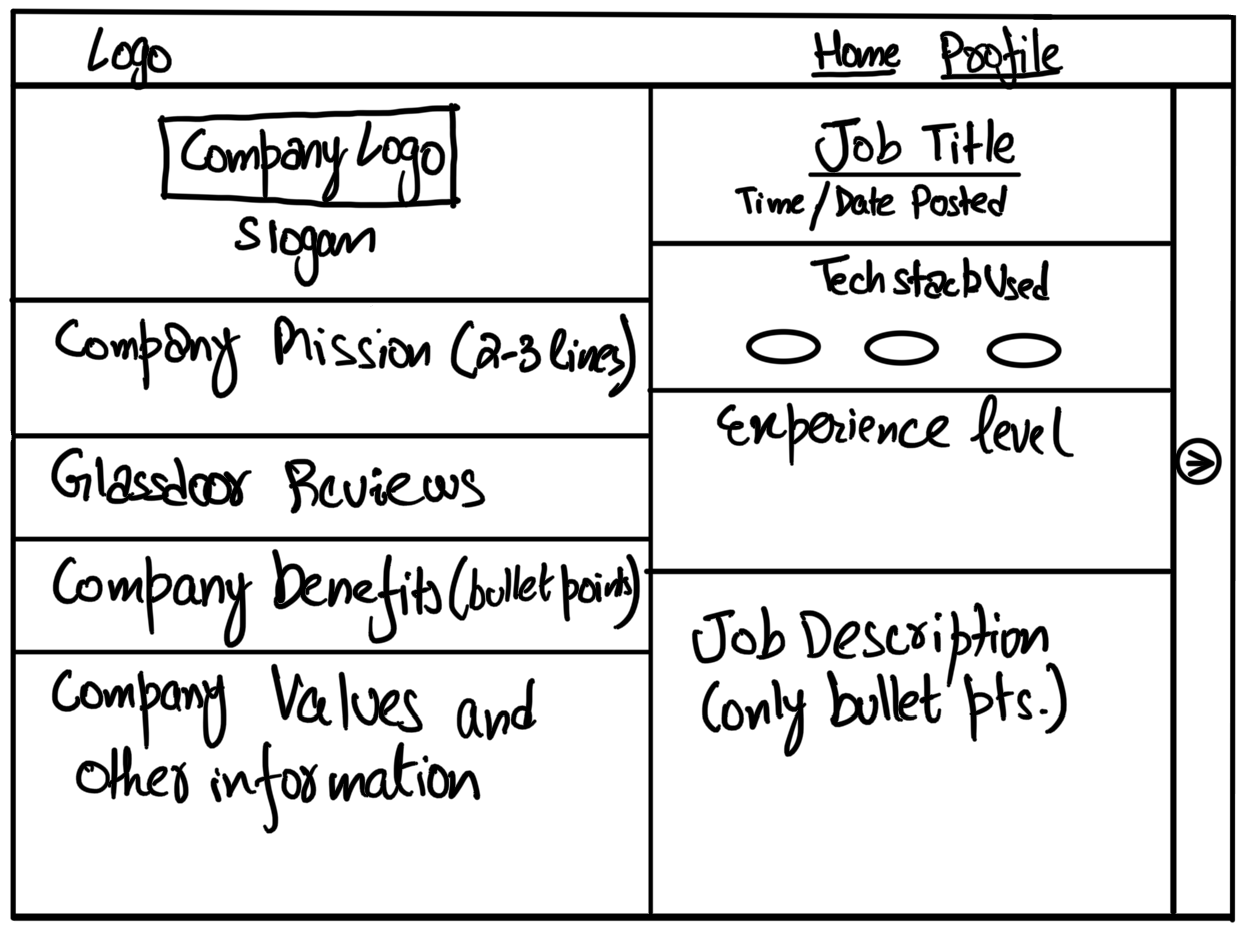
\includegraphics[width = 140mm]{Figures/lowfidelityprototype.png}
    \decoRule
    \caption[Low-Fidelity Prototype of the web app]{Low-fidelity Prototype of a job posting on the app}
    \label{fig:Low fidelity Prototype of a job posting on the app}
\end{figure}

These were the main reasons and justification behind building this web app. 

\newpage
\section{Current Applications}
There are many popular job search engines on the internet, and below is the current research on the most used ones \parencite{Reference1}.

\subsection{Indeed}
As of September 2021, Indeed is the number one job site in the world \parencite{Reference2} and is the reason why this research needs to begin with this web-app. Indeed's statistics show that during the period of April-September 2022, there were about 300 million unique visitors on the platform each month \parencite{Reference3}. Indeed has become this popular due various reasons one of which was due to its correct entry to the market in 2004 before which applying to jobs mostly happened offline and because it was free to use. The success of Indeed is due to two main reasons: 
\begin{itemize}
    \item It's Fast and Free for employers: About 43 percent of job openings are filled within the first 30 days, according to a new report from Indeed and the Centre for Economic and Business Research (CEBR). And the 57 percent of job openings that aren’t filled during that first month will likely remain unfilled for three months or more \parencite{Reference7}. Using Indeed is also free of cost so business owners on a tight budget don't need to spend a penny to post a job on Indeed. 
    \item Just Jobs for applicants: Going into the Indeed website, even if you're not logged in, shows the user just two fields to enter: "What?" and "Where?". Entering those will provide the user with all the jobs related. This helps users find the job they want quickly without having to go through all the trouble of logging in before looking for a job like it's competitors like LinkedIn, GlassDoor, etc. 
    \begin{figure}
        \noindent
        \centering
        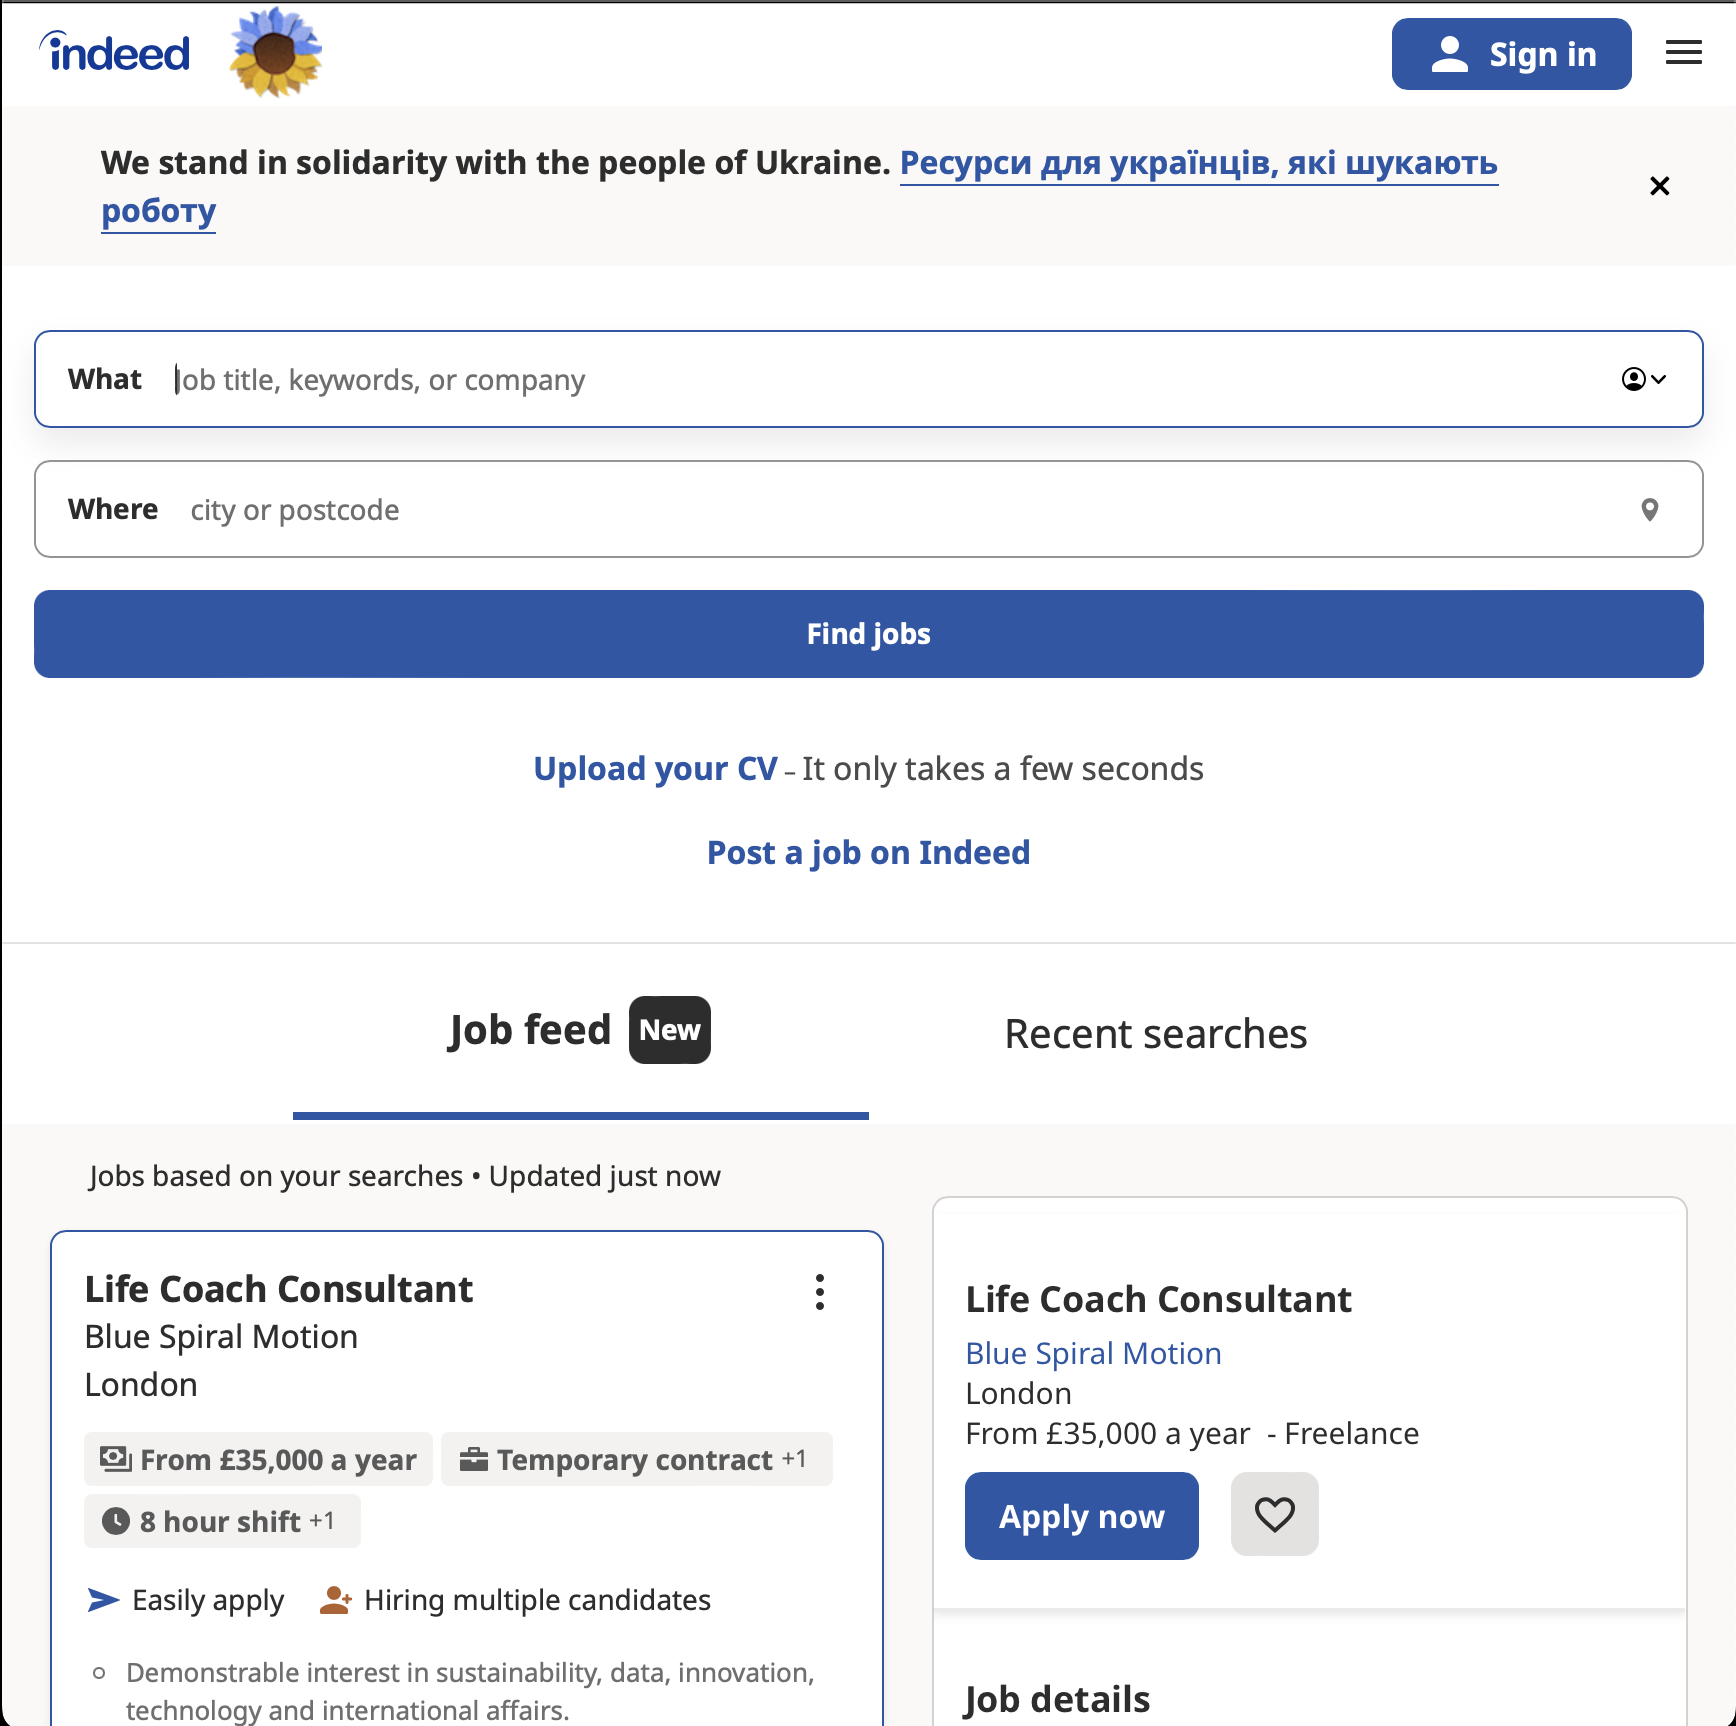
\includegraphics[width = 140mm]{Figures/IndeedHomepage.png}
        \decoRule
        \caption[Indeed's Homepage]{The Homepage of Indeed as of November 2022}
        \label{fig:Indeed Homepage}
    \end{figure}
\end{itemize}

So where does Indeed get it wrong? The main problem with the website is that it is overloaded with jobs. Just searching for a job will provide the user with an enormous list often in the tens of thousands vaguely relevant to their skill set and interests. It's clear to see that Indeed favours quantity over quality. Going by the reviews \parencite{Reference8} on multiple websites, it's clear to see that the users are generally dissatisfied with Indeed. Indeed has a rating of 1.5 on Trustpilot with 4,559 reviews as of November 2022 \parencite{Reference9}. It's clear to see that most users are not happy with the most used job search engine.

\subsection{LinkedIn}
Currently having over 875 million people \parencite{Reference10}, LinkedIn is one of the best places to start networking and reaching out to professionals of different ages and backgrounds related to your career. LinkedIn is a great place to follow different companies a user is interested in and see what they are up to, as well as create a profile for recruiters to look at when they apply for a job. 

However, due to all this networking, LinkedIn is considered more of a social media platform than a job board. This explains why users are redirected to their feed rather than LinkedIn's job search page when they log in to LinkedIn. LinkedIn is also considered the "new Facebook" with tools such as reacting to different posts on your feed like Facebook. LinkedIn is said to be "morphed from a CV Resource to a social media hub" \parencite{Reference14}. An article from the Guardian considers maintaining their LinkedIn page the equivalent of "cleaning their cutlery drawers or wiping down light bulbs – you do it irregularly and perfunctorily because someone told you to, not because there is any obvious benefit." \parencite{Reference11}. Multiple articles suggest that users use LinkedIn because "someone told them to" \parencite{Reference12}. Searching for jobs, on the other hand, is another story. A statistic shows that only 41\% of LinkedIn users thought LinkedIn helped them discover potential job opportunities \parencite{Reference13}. 

What is LinkedIn used for, then, if not for jobs? LinkedIn is considered one of the best tools for networking. It is a great tool to keep in touch with old colleagues and connect with new ones as you go through your professional career, but the future of LinkedIn is not painting an incredible picture for the job seeker.

\begin{figure}
    \noindent
    \centering
    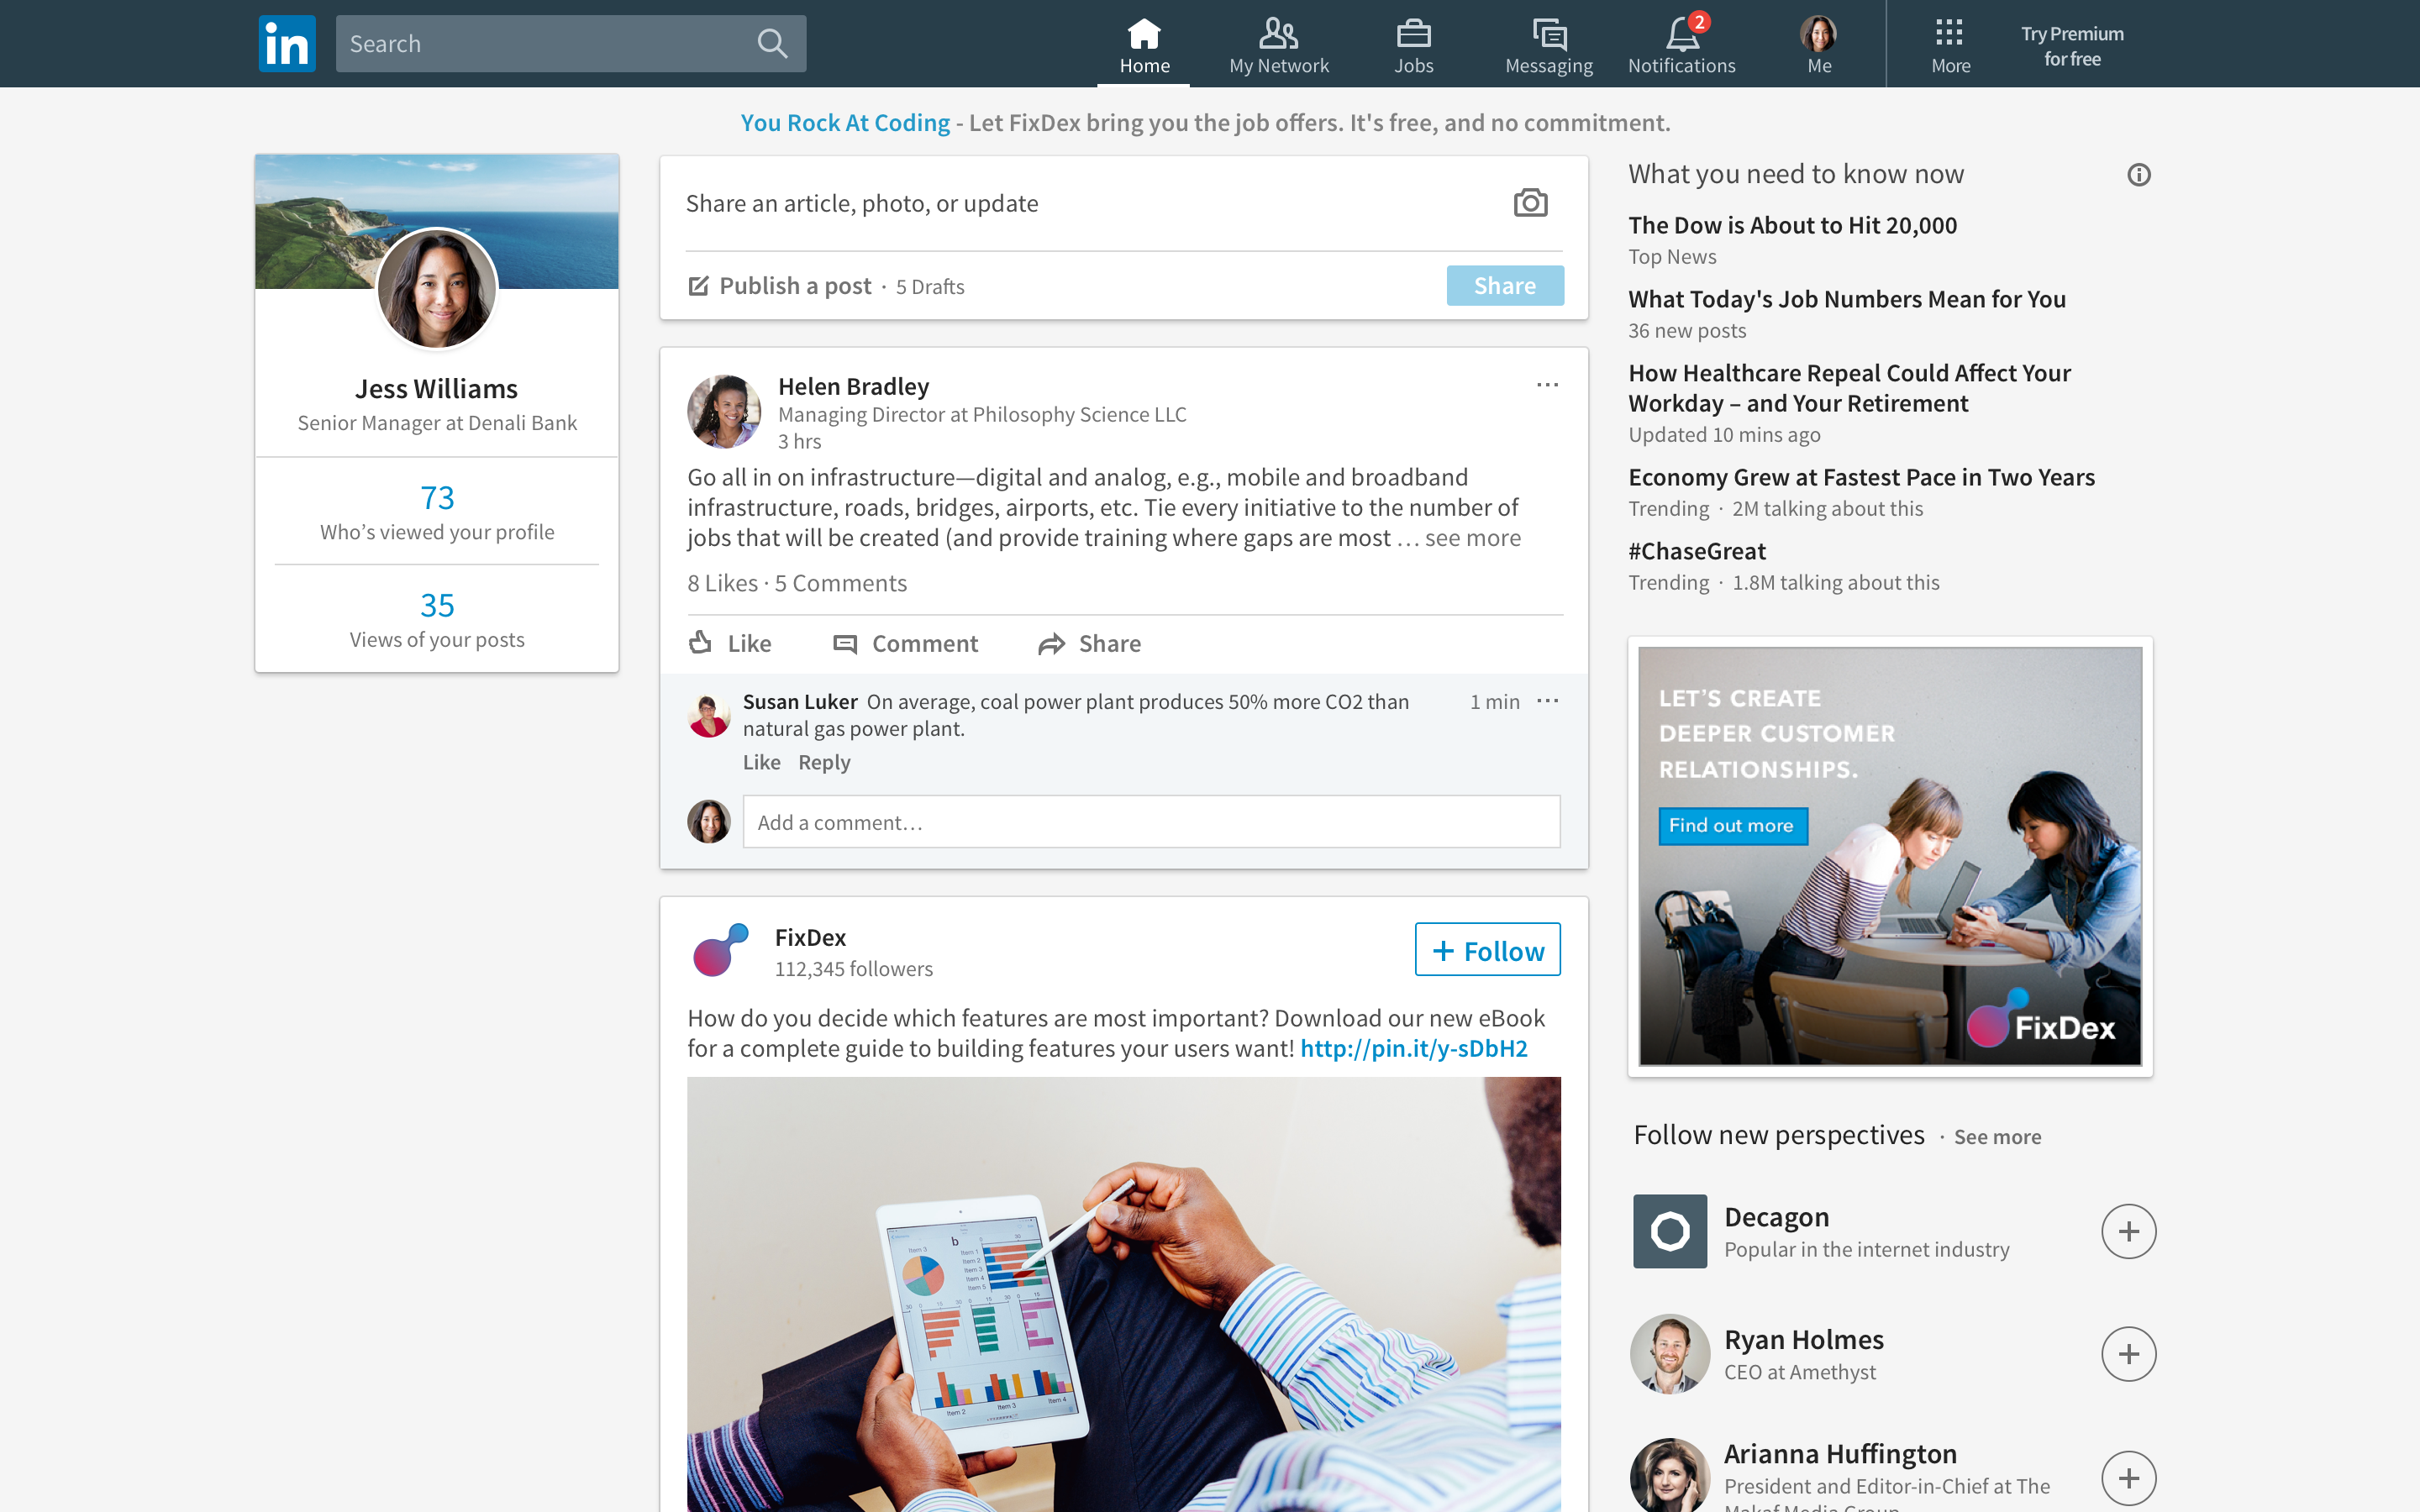
\includegraphics[width = 140mm]{Figures/LinkedInHomepage.png}
    \decoRule
    \caption[LinkedIn's Feed]{The Homepage of LinkedIn as of November 2022}
    \label{fig:LinkedIn Homepage}
\end{figure}

\newpage
\subsection{CareerBuilder}
CareerBuilder is another job search engine that resembles Indeed in several ways. CareerBuilder's homepage has the same two questions (What? and Where?) as Indeed's; however, where it does not resemble Indeed is the price. While Indeed is free to post jobs and look for them, CareerBuilder charges a hefty £349 for their cheapest lite tier, which includes 10 Resume Actions for a day limit \parencite{Reference15}. CareerBuilder does not have any free tier for employers, and as a reason, it is only in the interest of companies which are in a hiring surge or large enough to need hires regularly. With a rating of just 1.48 stars, it is clear that employers and employees alike do not seem to like the product. Users reported getting much spam after registering with CareerBuilder \parencite{Reference16}.

\begin{figure}
    \noindent
    \centering
    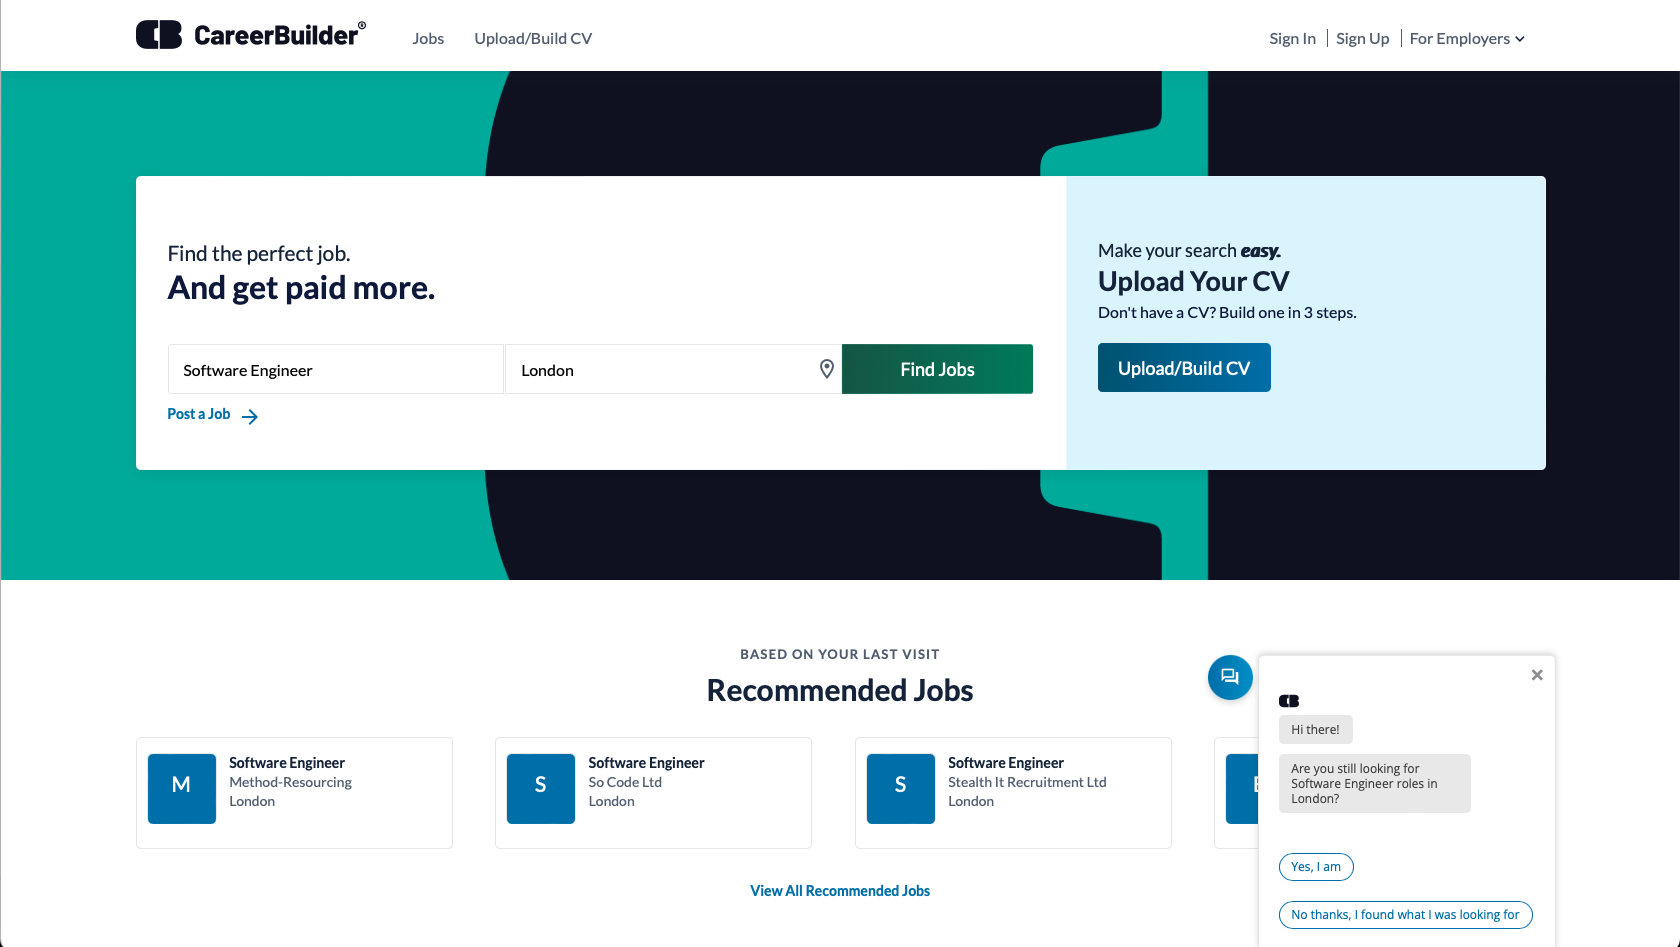
\includegraphics[width = 140mm]{Figures/CareerBuilderHomepage.png}
    \decoRule
    \caption[CareerBuilder's Homepage]{The Homepage of CareerBuilder as of November 2022}
    \label{fig:CareerBuilder Homepage}
\end{figure}

\subsection{Glassdoor}
Glassdoor started as a ratings and reviews web app where employees could leave anonymous reviews to employers. Through the years, Glassdoor has grown, and they now offer a job search engine where users can search for jobs using different filters like salary, employee satisfaction, etc. Unlike Indeed and CareerBuilder, users need to register to search for jobs, but it is free to use. In 2018, Glassdoor was acquired by Indeed's parent company for \$1.2bn making them sister companies. As a result, jobs are shared between both platforms. \parencite{Reference17}

While it can now be used as a job search engine, Glassdoor was mainly designed and developed as a ratings and reviews web app; most users use it for just that. Job seekers mostly use Glassdoor to evaluate a company's work environment, salary and other things, not to look for jobs.

\begin{figure}
    \noindent
    \centering
    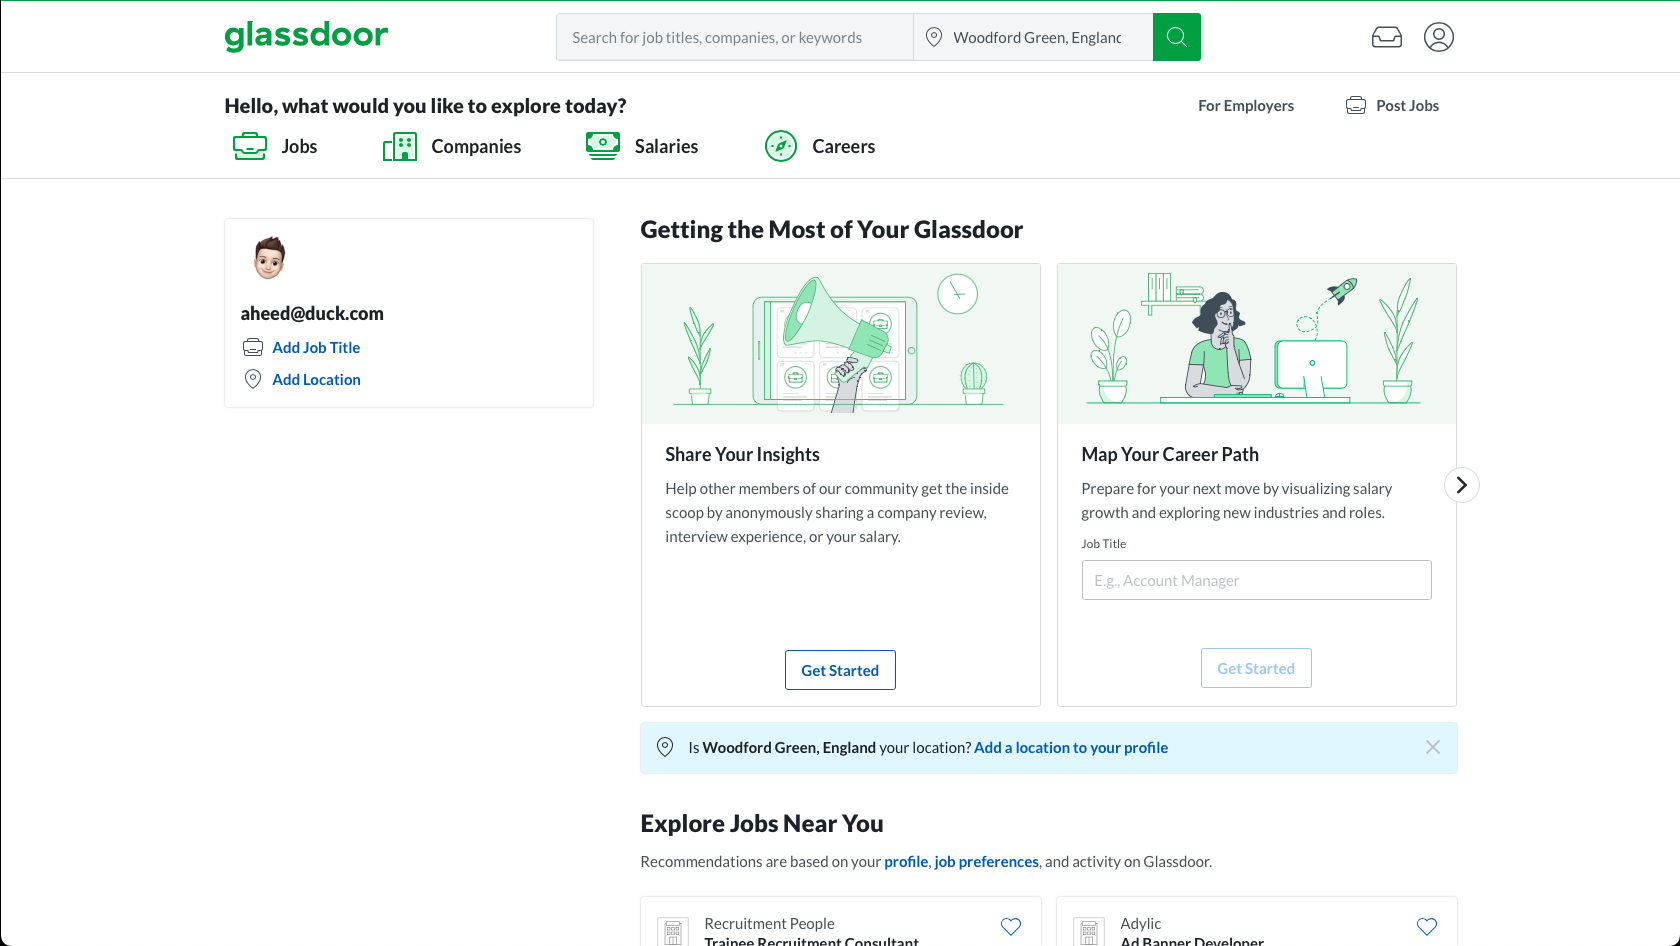
\includegraphics[width = 140mm]{Figures/GlassdoorHomepage.png}
    \decoRule
    \caption[Glassdoor's Homepage]{The Homepage of Glassdoor as of November 2022}
    \label{fig:Glassdoor Homepage}
\end{figure}

\section{Tools and Technologies}
As the development stage of the web app is yet to begin, the tools and languages used to build this application are not definite, but more tools will be added to the application as required. Below is a list of tools and languages with which the development stage will begin. Additional knowledge about these technologies or others will be learnt from online courses through Udemy \parencite{Reference25}, Coursera \parencite{Reference26} or other websites. 

The language used to build this software will be: React, HTML, SASS. The reason why these languages are chosen is because:

\begin{itemize}
    \item \textbf{React:} \parencite{Reference20}
    \begin{itemize}
        \item Reusable Components: One of the main advantages of React is that you can reuse components. It saves much time as you do not have to code the same feature again, and you can reuse them.
        \item Speed: React minimises DOM changes, making it highly efficient and providing excellent performance to users.
        \item Easy to Test: React provides its testing library, making it really easy to test its components.
        \item Familiarity: React is very similar to JavaScript, which makes it familiar to Native JavaScript.
    \end{itemize}
    \item \textbf{HTML5:} \parencite{Reference21}
    \begin{itemize}
        \item HTML code will be used inside react components to make them reusable.
        \item HTML ensures the proper formatting of text and images for any Internet browser.
    \end{itemize}
    \item \textbf{SASS:} \parencite{Reference22}
    \begin{itemize}
        \item SASS contains all the CSS features and more features not present in CSS, making it a good choice for developers to use.
        \item SASS offers variables; you can shorten your code by using variables. It is a great advantage over conventional CSS.
    \end{itemize}
    \item \textbf{Firebase:} \parencite{Reference24}
    \begin{itemize}
        \item Authentication SDK using Firebase is very easy, and many features like "Sign in using Google" or "Sign in with Apple" can be used easily through Firebase.
        \item Firebase provides a free tier with many features perfect for this web app, including 100 simultaneous connections fit for an MVP of this product.
    \end{itemize}
\end{itemize}

To use all these languages, you need a tool that works well with all of them and IntelliJ IDEA Ultimate Edition \parencite{Reference23} was fit for these languages. It contains countless extensions with which using these languages becomes easy. 

Version Control is essential to all developers, even when you are working alone. The peace of mind you have when you know a working backup if safe is essential for a developer. For version control, this project will be regularly uploaded to GitHub to keep track of changes.

As Agile Methodologies will be used during the development stage of this software, Jira by Atlassian \parencite{Reference27} will be used to create Sprint boards to help keep track of the progress of the development of software as well as any bugs which pop up during the development of this app. Along with this, different milestones will also be created to help keep track of the project. 

\section{Summary}
It was beneficial to research existing applications on the internet that job seekers use to look to begin or further their careers. It helped identify the key features of what this app should have to make it one of the best in the market for tech jobs. The main points for this application that should stand out were:

\begin{itemize}
    \item \textbf{No endless scrolling:} This app will show jobs designed loosely like a pamphlet where every bit of information is in bold and in front, and users will have the option to apply for the job or skip to the next one (See Figure \ref{fig:Low fidelity Prototype of a job posting on the app}). 
    \item \textbf{A reply back:} A poll suggests that 62\% of applicants spend at least 30 minutes on their application, and 38\% spend up to 30 minutes on an application. \parencite{Reference18}. Every applicant who spends time sending an application for a job deserves a reply from companies. This app, in addition to sending an email when applying for a job, will send one as soon as the job is marked as filled by the recruiter or taken down from the platform.
    \item \textbf{Reinventing job descriptions:} Job descriptions need to be rethought. Going through job descriptions in tech is a nightmare. The need to scroll down all about the company's profile to find what tech stack they use or what the level of the job applicant should be (entry-level, mid-level or senior level). This app will solve it by keeping separate tags below the job title, which should point out the technologies/languages the company uses. (See Figure \ref{fig:Low fidelity Prototype of a job posting on the app})
    \item \textbf{No Outdated jobs:} One of the main criticisms in the online job search industry is that they include many outdated jobs. Job Crop should be different in this regard. Jobs will not be shown on the platform after 15 days. If the job is still open and the recruiters have yet to find a candidate, they will get an option to keep the job on the platform for another 15 days if they wish to do so.
    \item \textbf{Only Jobs in tech:} Job search engines like LinkedIn have strayed away from being what a job search engine should be: Just jobs. This app will be built on the foundation that users would come to this app for just one thing: A job in the tech industry.
\end{itemize} 
\chapter{Design}
The system's design is critical to understand the project and an important metric to measure the project's success. This section entails the design process of different system parts and the application's high-fidelity prototypes.

\section{Research behind the design}
The design of this web app was done keeping in mind the summary of the background research. To make sure the requirements set in the background research were met, further research was needed to fulfil these requirements.

\subsection{Questionnaire for applicants}
To ensure that the jobs shown on the job applicant's side match their requirements and what they are looking for in a role, they will be asked questions when signing up for this application. These questions will all be multiple-choice or tag-based, which will be less time-consuming for applicants and easier for them simultaneously. The time taken by these questions should ideally be lesser than three minutes. These questions would then help match the applicants to job applications. 

It is also essential to choose the right questions to ask the applicants and have certain restrictions on the questions having tags to prevent users from selecting many of them. The questions asked to applicants are based on the mix of questions an employer looks for in an employee and vice-versa. \parencite{Reference28}

Questions asked to users would be:
\begin{enumerate}
    \item \textbf{Which city would you like to work in?} This will include a remote option and top cities throughout the United Kingdom.
    \item \textbf{What role do you want to work in?} This question will be tag-based, with many answers an applicant can choose from. A follow-up question will be asked based on this option, in which the applicant will choose the role most relevant to them. For example, suppose an applicant selects Software Engineering. In that case, they will get multiple roles in Software Engineering like Back-end engineer, front-end engineer, DevOps Engineer, Game Engineer, etc., which they can choose from. This will make it easier for the application to match them with the relevant role. A restriction of a maximum of three positions will be put in place for this answer.
    \item \textbf{What level of a job are you looking for?} Multiple answers with a restriction of a maximum of two will be given for this question. Internships, Entry-level jobs, Senior-level jobs, etc., will be answers a user can select.
    \item \textbf{What  are your favourite technologies?} An applicant will be given a tag-based question where they can select the must-have technologies and nice-to-have technologies. 
    \item \textbf{What technologies do you not like?} Here, an applicant will be again given a tag-based question where they can select the technologies they don't want to use in their future role.
    \item \textbf{When can you start?} This will have multiple options, including: In the following year, As soon as possible, I just want to have a look, etc.
    \item \textbf{Minimum expected salary?} In this question, the applicant can enter the minimum salary they would be expecting for the roles they would apply for. 
    \item \textbf{Do you need a visa to work in the UK?} This will be a Yes or a No question. Jobs which do not sponsor applicants to work in the UK will be hidden or shown based on this answer.
\end{enumerate}

Similar questions will be asked of employers for each job they post on the platform. Employers must answer these questions, which will let the application match the employers to the applicants based on the job and the job applicant's requirements. 

\section{System Requirements}
A set of requirements for each component of the project are defined below to ensure the aims, objectives and design requirements of the project are met.

\subsection{Front-End Requirements}
To make the application appealing and eye-catching, the front end needs to look modern, only having necessary details and not overloaded with information.

To ensure that these conditions are met, the front end needs to have the \break following:
\begin{enumerate}
    \item An appealing website home page: The homepage should be able to grab the attention and create a first impression on the user as soon as they open it. 
    \item Optimised for mobile phones: Users should be able to open and use the website on their mobile phones.
    \item A login page for job applicants and employers to access specific website pages.
    \item Specific routes which require logging in should not be accessible to users not logged in.
    \item Allow users to log in and log out of the website.
    \item Allow easy navigation from web pages.
    \item Have an interactive design for users.
\end{enumerate}

\subsection{Back-End Requirements}
An algorithm is needed to match the data provided in each job to the applicant's requirements. This algorithm will be used in the back end, written in JavaScript.

The requirements for the back end of this application are:
\begin{enumerate}
    \item Match jobs with applicants using an algorithm which matches the job's requirements to the applicant's requirements.
    \item Efficiently read the data from the front end and output the necessary data to the user side.
    \item Write readable code for other developers to grasp quickly.
\end{enumerate}

\subsection{Database Requirements}
The database, MySQL in this case, will store information of all users, including different jobs, user information, etc. 

The database requirements for this application are:
\begin{enumerate}
    \item Store data of users securely in the database using algorithms like hashing to ensure the data is secure even through a data breach. \parencite{Reference29}
    \item The database should allow quick and easy data retrieval.
    \item Reduce redundancy in the database, leading to slow data retrieval and unnecessary information.
\end{enumerate}

\subsection{Functional Requirements}
The functional requirements of this application are needed to identify what the system should achieve for users to do their tasks and also to understand any limitations this application might have. Functional requirements, defined below, are the minimum standard for what the application should be able to do for users to achieve their tasks and use this web app efficiently.

The research done into creating an app such as this has resulted in the following functional requirements:
\begin{enumerate}
    \item This application should be able to run on different browsers and mobile phones as well.
    \item It should be able to store the user data on the database securely and allow users to log in and register for this web app.
    \item The application should stay logged in for a specific time if the user has not logged out, even if the user has closed the browser.
    \item The application should provide an interface of different jobs to applicants which they can choose from.
    \item The application should allow employers to register their companies and add jobs.
    \item The application should be able to send an automated email to users each time they apply for a job and when they register for a job. 
\end{enumerate}

\subsection{Non-Functional Requirements}
The non-functional requirements can be used to judge the operation of a system. These are as follows:
\begin{enumerate}
    \item The matching algorithm which matches the jobs to the applicants should not take longer than 5 seconds.
    \item Each page must load within 2 seconds.
    \item The system must meet Web Content Accessibility Guidelines. \parencite{Reference30}
    \item The application's interface has to be user-friendly and easy to use.
\end{enumerate}

\subsection{User Requirements}
The user requirements contain the basic things users should be able to do in the MVP. These are as follows:
\begin{enumerate}
    \item Job applicants should be able to see jobs that match their requirements
    \item Job applicants should be able to edit their answers to the "quiz" based on the change of requirements they have through their careers.
    \item Users should be able to log in and register, and a display message should pop up if a wrong password/username is given.
    \item Employers should be able to add a new job to the platform.
    \item Employers should be able to see the applicant's profile, including their resume and other data the applicant wants to share with them.
\end{enumerate}

\section{System Design}
This section consists of the database design, which will be used in this application to store data, Use Case diagrams which constitute different user journeys and some designs and wireframes for this application. 

\subsection{Database Design}
The database design is an essential component for this application to store and use the data provided by users in the web application. A good database design also makes locating information in the web app easier and is crucial in efficiently executing queries and ensuring information consistency. For these reasons, the database must be correctly designed to make it easier to locate information and reduce redundancy.

\subsubsection{Entity Relationship diagram}
An ERD is used to visualise the relationship between each table in the database. It is essential to design an ERD before creating it as it helps debug future bugs and identify any design flaws before and during the development stage. Each row in every table should also have the correct data type for each column in SQL to determine what kind of data is expected inside each column and to ensure that accurate information is stored inside each table.

The ERD created contains two main tables which have the user's information. This is the information that isn't changed often and isn't directly linked to the specification of a job. A job applicant's name, LinkedIn URI and Rèsumè/CV are a part of this table. This table can add multiple rows as the application grows, but this information is sufficient for the MVP. 

Similarly, for Employers, the data that doesn't frequently change, like the company logo or slogan, is part of the top-level table called employers. Under this table, different jobs are created, which can then be matched to the user requirements in the back end of the application. No direct relation is needed between applicants and employers as this will be done at the back end of the application.

The relationships of different tables are shown below:
\begin{enumerate}
    \item Applicant Information to Applicant Requirements: This is a one-to-one relationship as an applicant is only allowed one set of requirements. The jobs the applicant gets shown will be dependent on these requirements. The user id is the key used in both tables to identify each row uniquely.
    \item Employers to Jobs: This is a one-to-many relationship as one company can create several jobs, each having different specifications and other requirements. The company id is the key used in all job tables and employers, which helps to identify the company that has put out the job uniquely.
\end{enumerate}


\begin{figure}
    \noindent
    \centering
    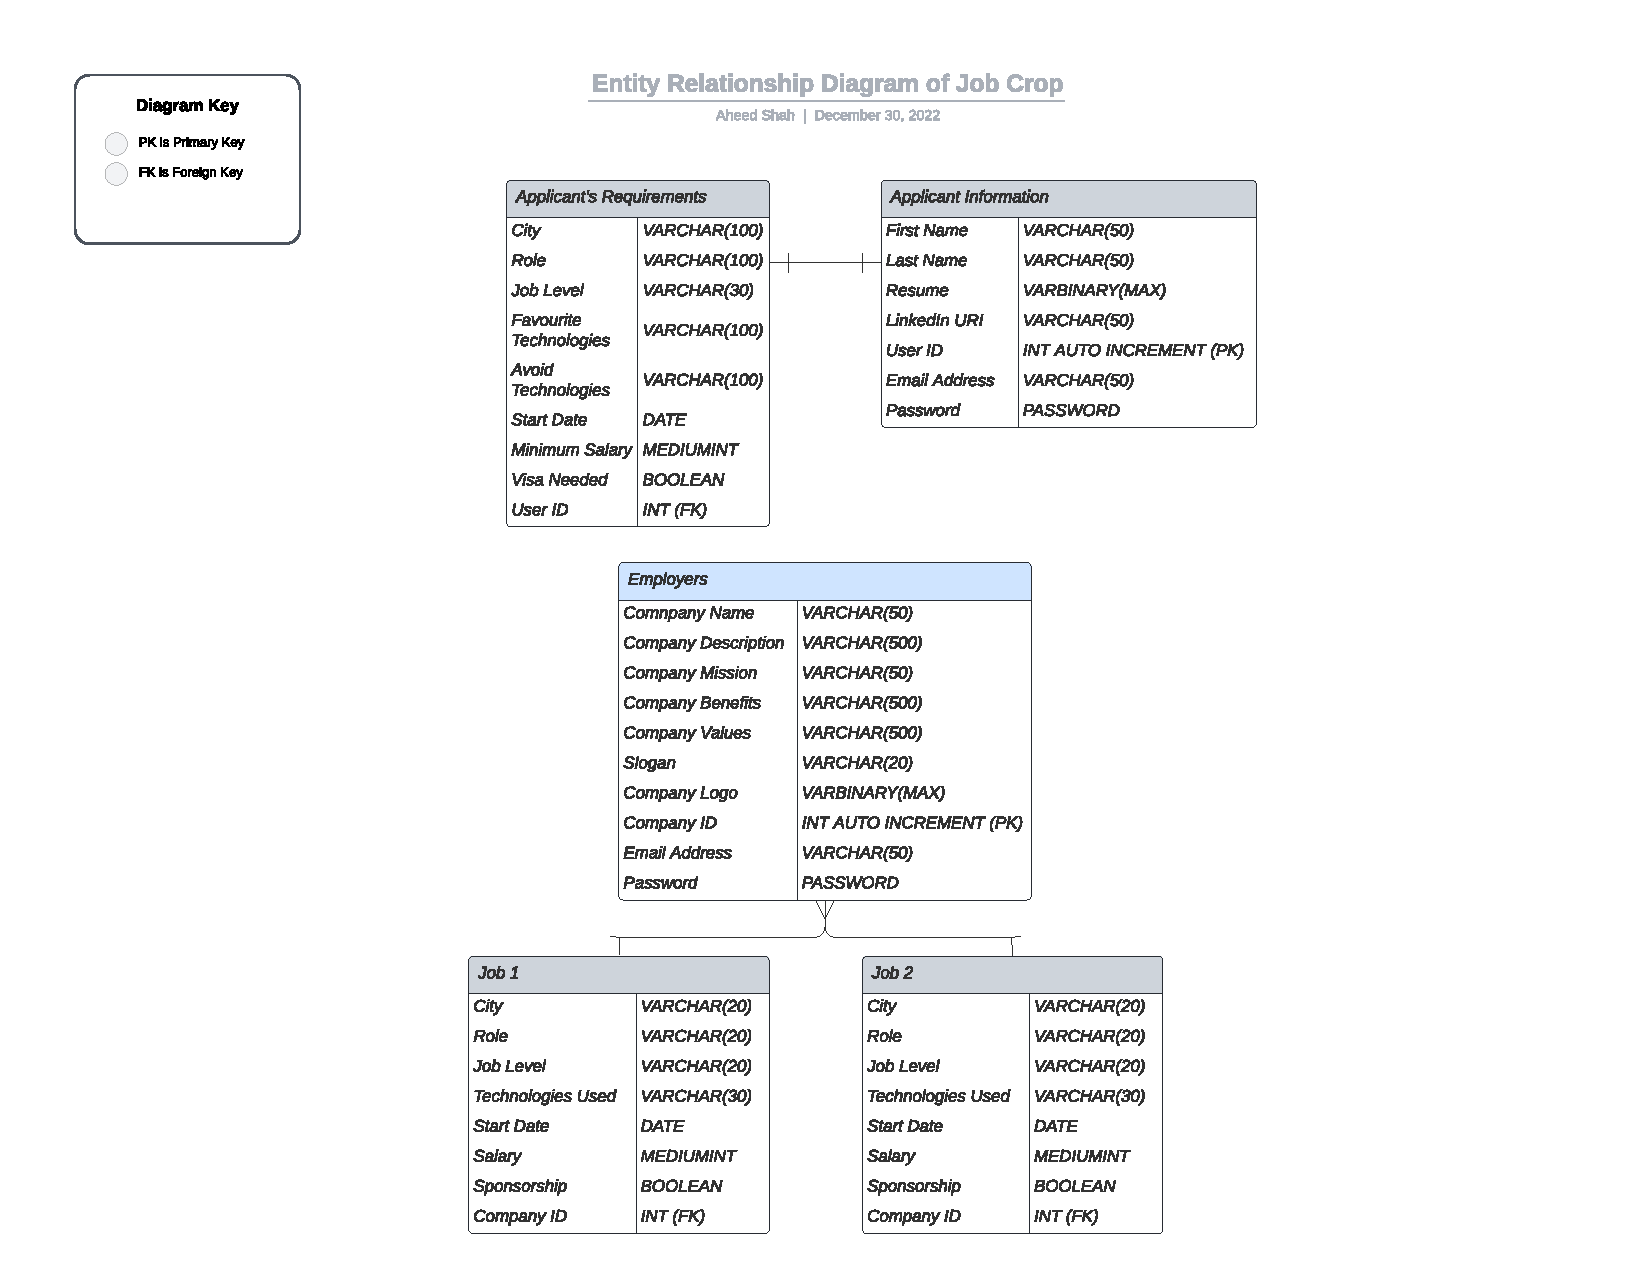
\includegraphics[width = 140mm]{Figures/ERD.pdf}
    \decoRule
    \caption[Entity Relationship Diagram]{Entity Relationship Diagram of the application}
    \label{fig: Entity Relationship Diagram}
\end{figure}

\subsection{Use Case Diagrams}
Use case diagrams specify the expected behaviour between the user and the application. These diagrams also help to visualise some of the different user journeys a user takes while using the application. 

Figure \ref{fig: Use Case Diagrams for Signing Up or Logging into the application} shows a user journey for a user to log in. If a user does not have an account with this application, they will be asked to sign up. Upon signing up and completing the questionnaire, they will be shown their specific matches based on these questions.

Figure \ref{fig: Use Case Diagram for applying for a job} shows a user journey for an applicant to apply for a job. It is similar to the previous user journey in the logging-in stage at first, but after the user gets shown different positions, they can apply for them or continue looking for another role. When they find the perfect role, they can click on the apply now button, which will allow them to continue to complete their application if there are any job-specific answers the employer needs the applicant to answer. As some jobs require users to go to specific companies' websites to apply, they can be redirected to that website to continue their application on a third-party website. The option to let users apply from this application, the company's own website, or both lies with the employer.

Figure \ref{fig: Use Case Diagram for an Employer to add a new job} shows a user journey of an employer adding a new job or looking through the applicants who have applied for the job posting. The use case diagram is quite similar in the login and sign-up stage, but employers get shown a different interface to look through the applicants for their previous job postings or the option to add a new job. To add a new job, an employer has to submit a similar questionnaire to what the applicant submits as their requirements. After this is successful, the job is added to the platform, and applicants can apply.

Creating these use case diagrams was quite helpful as the critical user workflows were thought about in detail when designing these workflows. It also helped outline the separate steps of different processes in sequential order. 

\begin{figure}
    \noindent
    \centering
    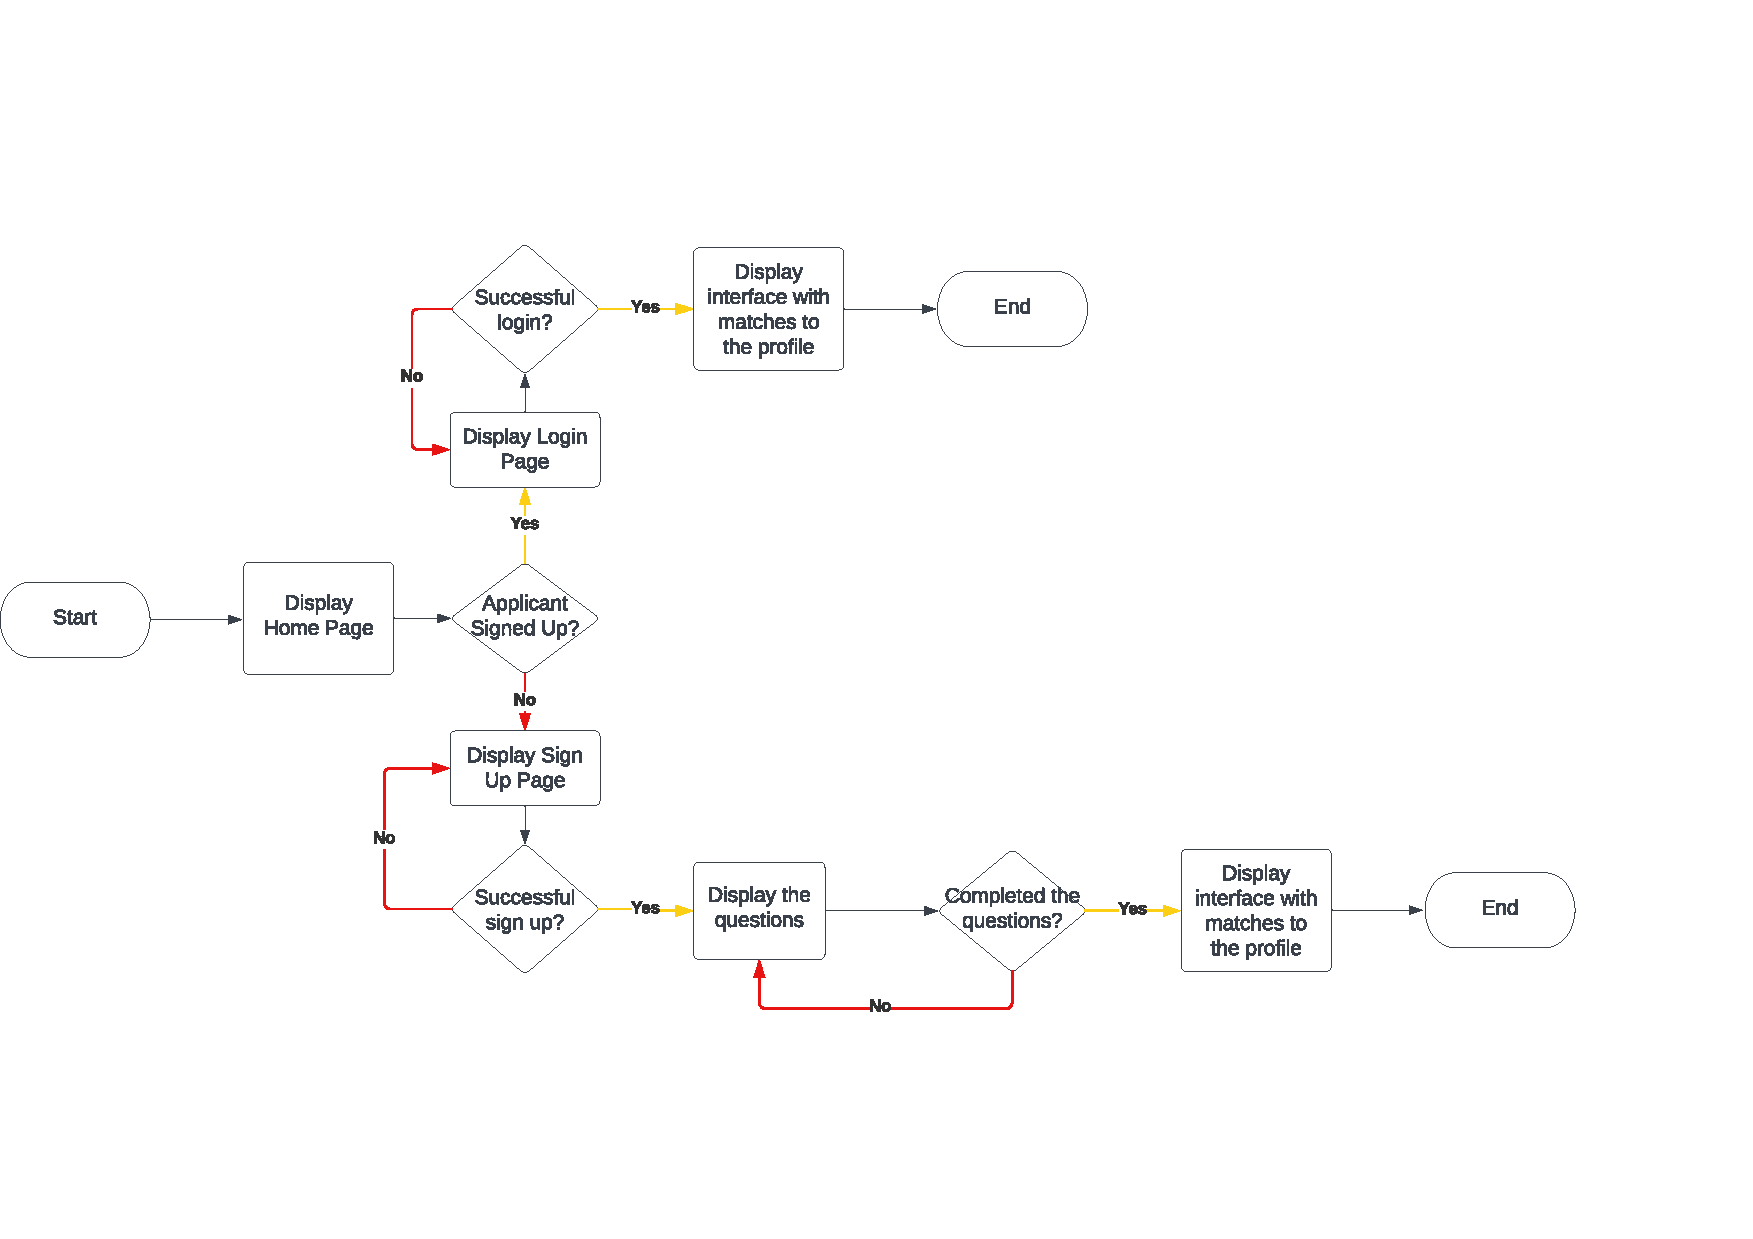
\includegraphics[width = 140mm]{Figures/signup.pdf}
    \decoRule
    \caption[Use Case Diagrams for Signing Up or Logging into the application]{Use Case Diagrams for Signing Up or Logging into the application}
    \label{fig: Use Case Diagrams for Signing Up or Logging into the application}
\end{figure}

\begin{figure}
    \noindent
    \centering
    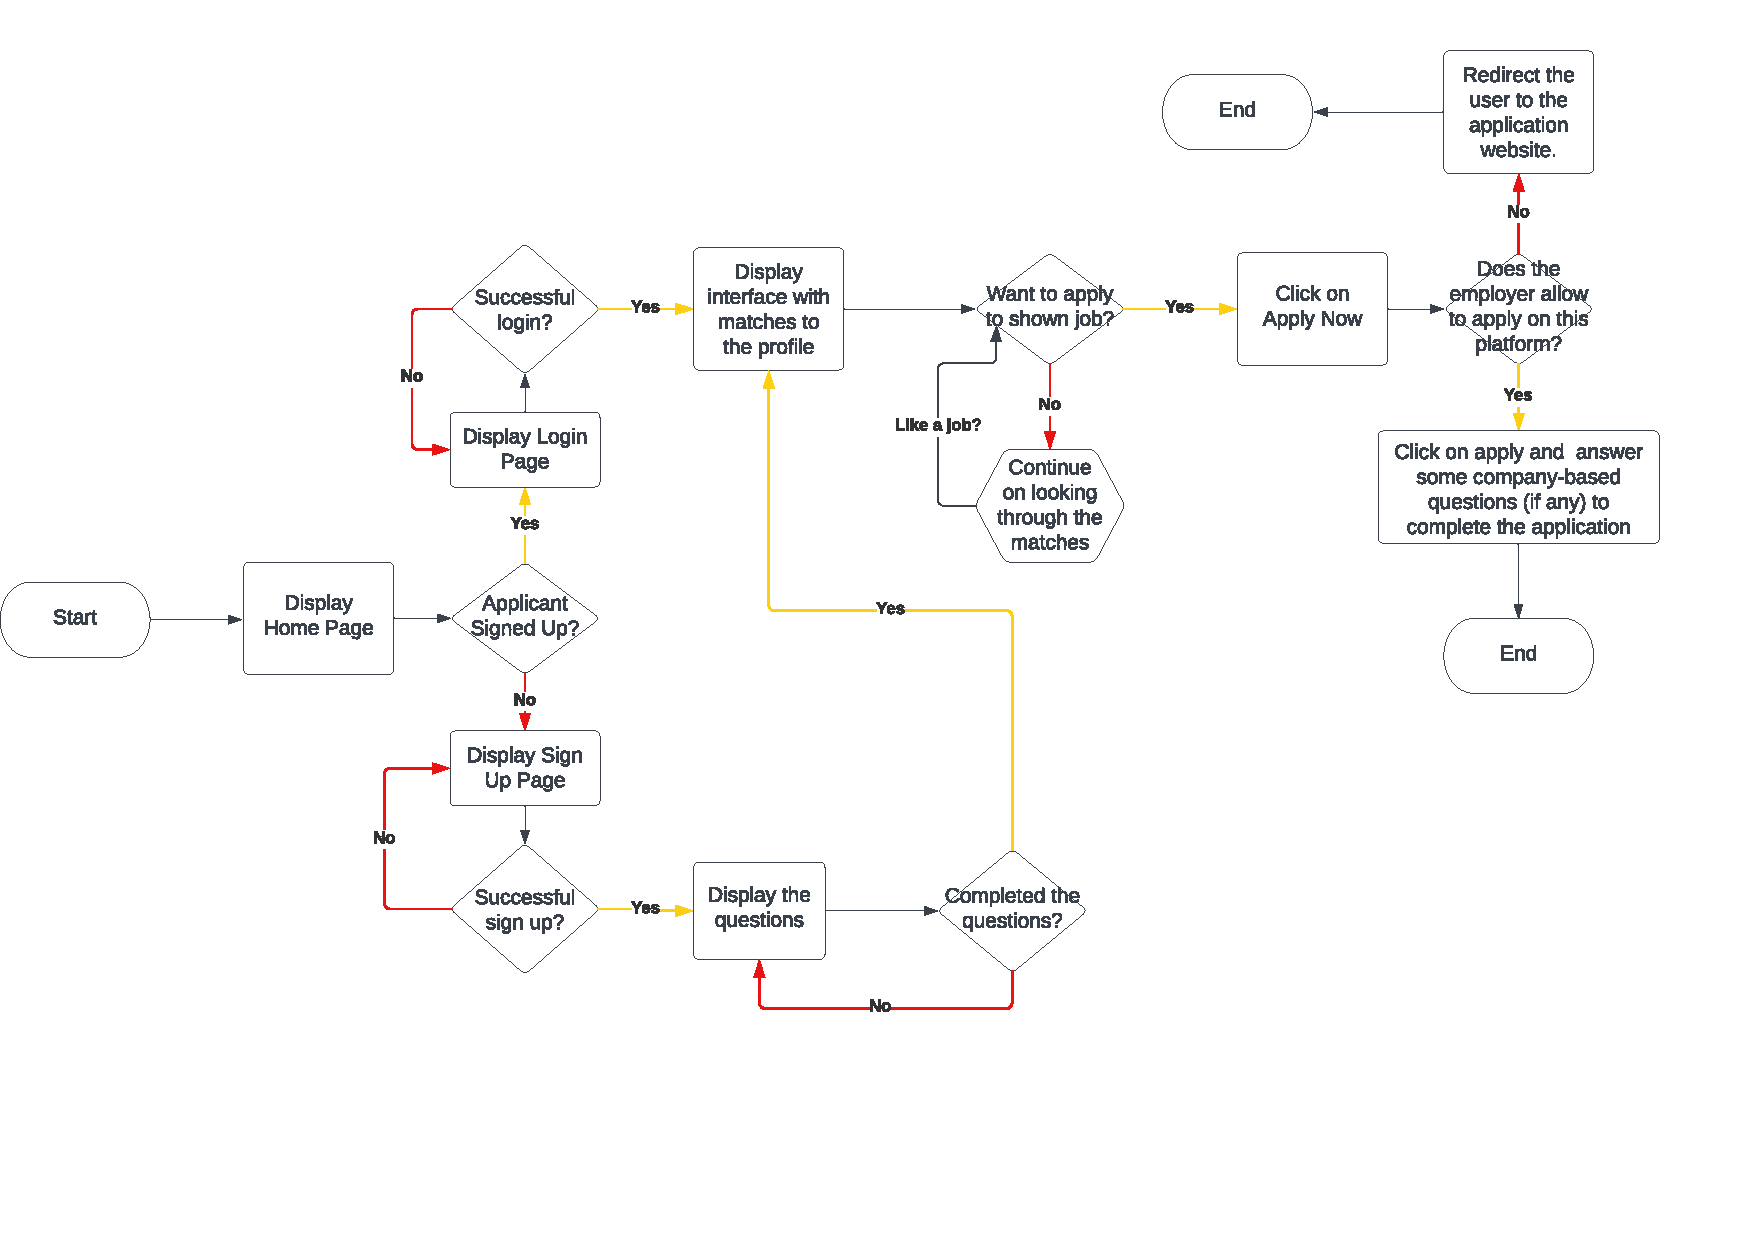
\includegraphics[width = 140mm]{Figures/applying.pdf}
    \decoRule
    \caption[Use Case Diagram for applying for a job]{Use Case Diagram for applying for a job}
    \label{fig: Use Case Diagram for applying for a job}
\end{figure}

\begin{figure}
    \noindent
    \centering
    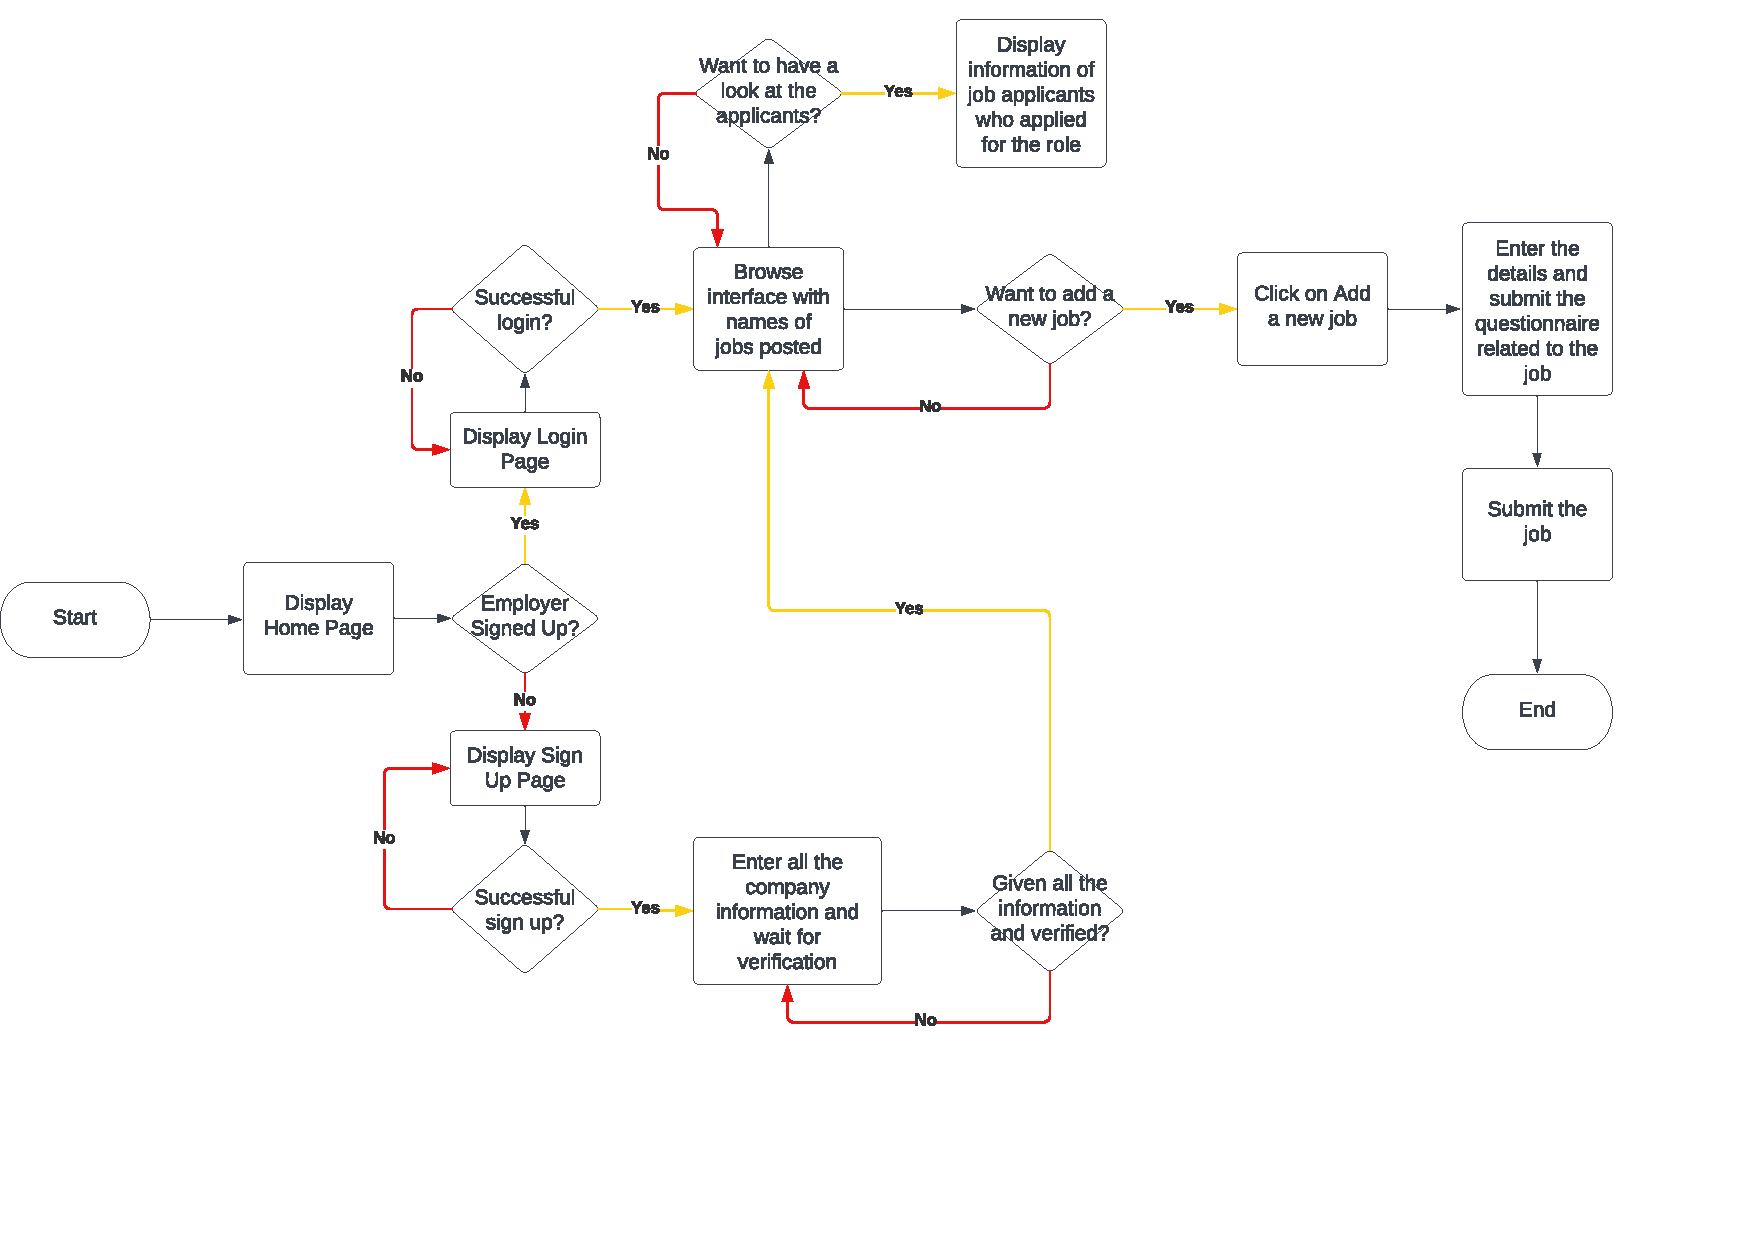
\includegraphics[width = 140mm]{Figures/employer.pdf}
    \decoRule
    \caption[Use Case Diagram for an Employer to add a new job]{Use Case Diagram for an Employer to add a new job}
    \label{fig: Use Case Diagram for an Employer to add a new job}
\end{figure}

\newpage
\subsection{Designs}
Some wireframes and designs were created to help visualise what specific pages will look like. This is the first prototype of these designs, which can be changed in the future based on user feedback. The goal of these is to create a simple design. 

The home screen shown in figure \ref{fig: Home Screen} shows the links on the header where applicants can click login to be redirected to the login page shown in figure \ref{fig: Login Page}. The home page still needs improvement, as some links aren't positioned where they should be, and some placeholder text is used in places. 

As shown in figure \ref{fig: Job Posting}, the job details are given on the right-hand side, and the company details are provided on the left-hand side. This helps users know which side to look for each component. Also, each section has a heading to make it even easier to find the details the applicant is looking for. The user can click on arrows on the right side to look at the next role or click on the arrow back to look at the previous job. If applicants want to apply, they can click on the apply button. Some design changes are needed on this page as the apply button isn't centred enough and doesn't seem appealing.

\begin{figure}
    \noindent
    \centering
    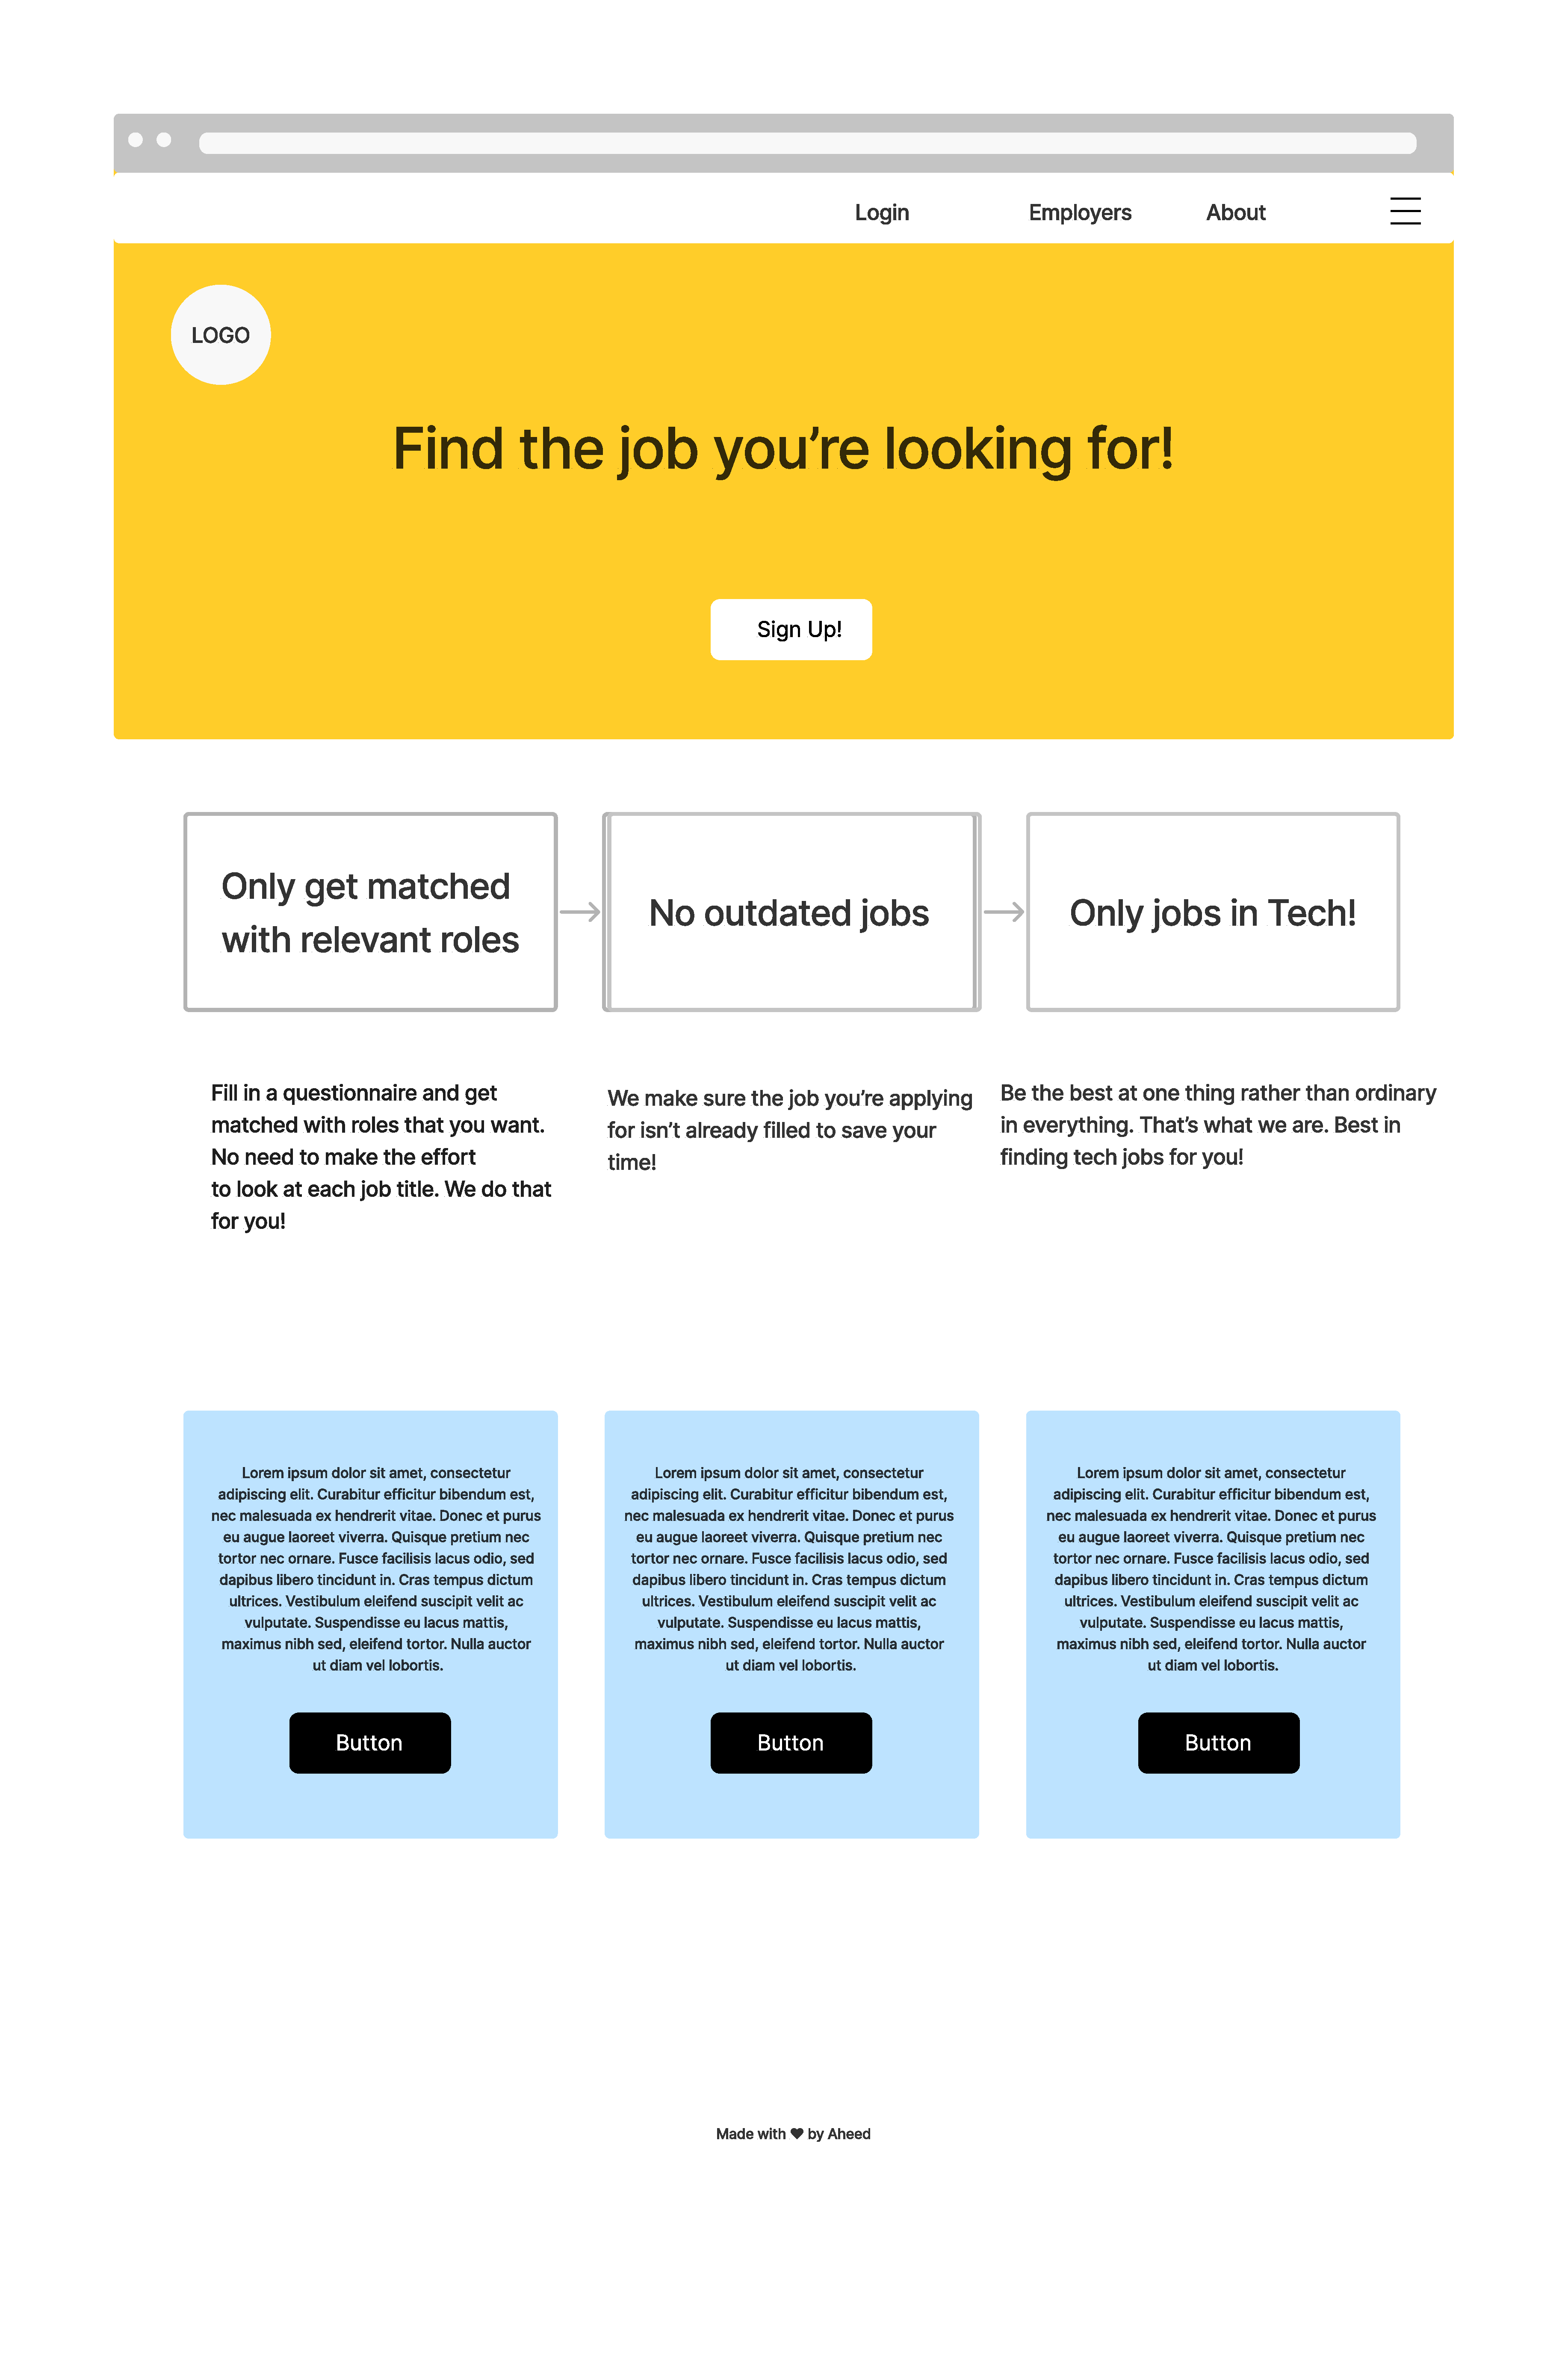
\includegraphics[width = 140mm]{Figures/homescreen.pdf}
    \decoRule
    \caption[Home Screen of the application]{Home Screen of the application}
    \label{fig: Home Screen}
\end{figure}

\begin{figure}
    \noindent
    \centering
    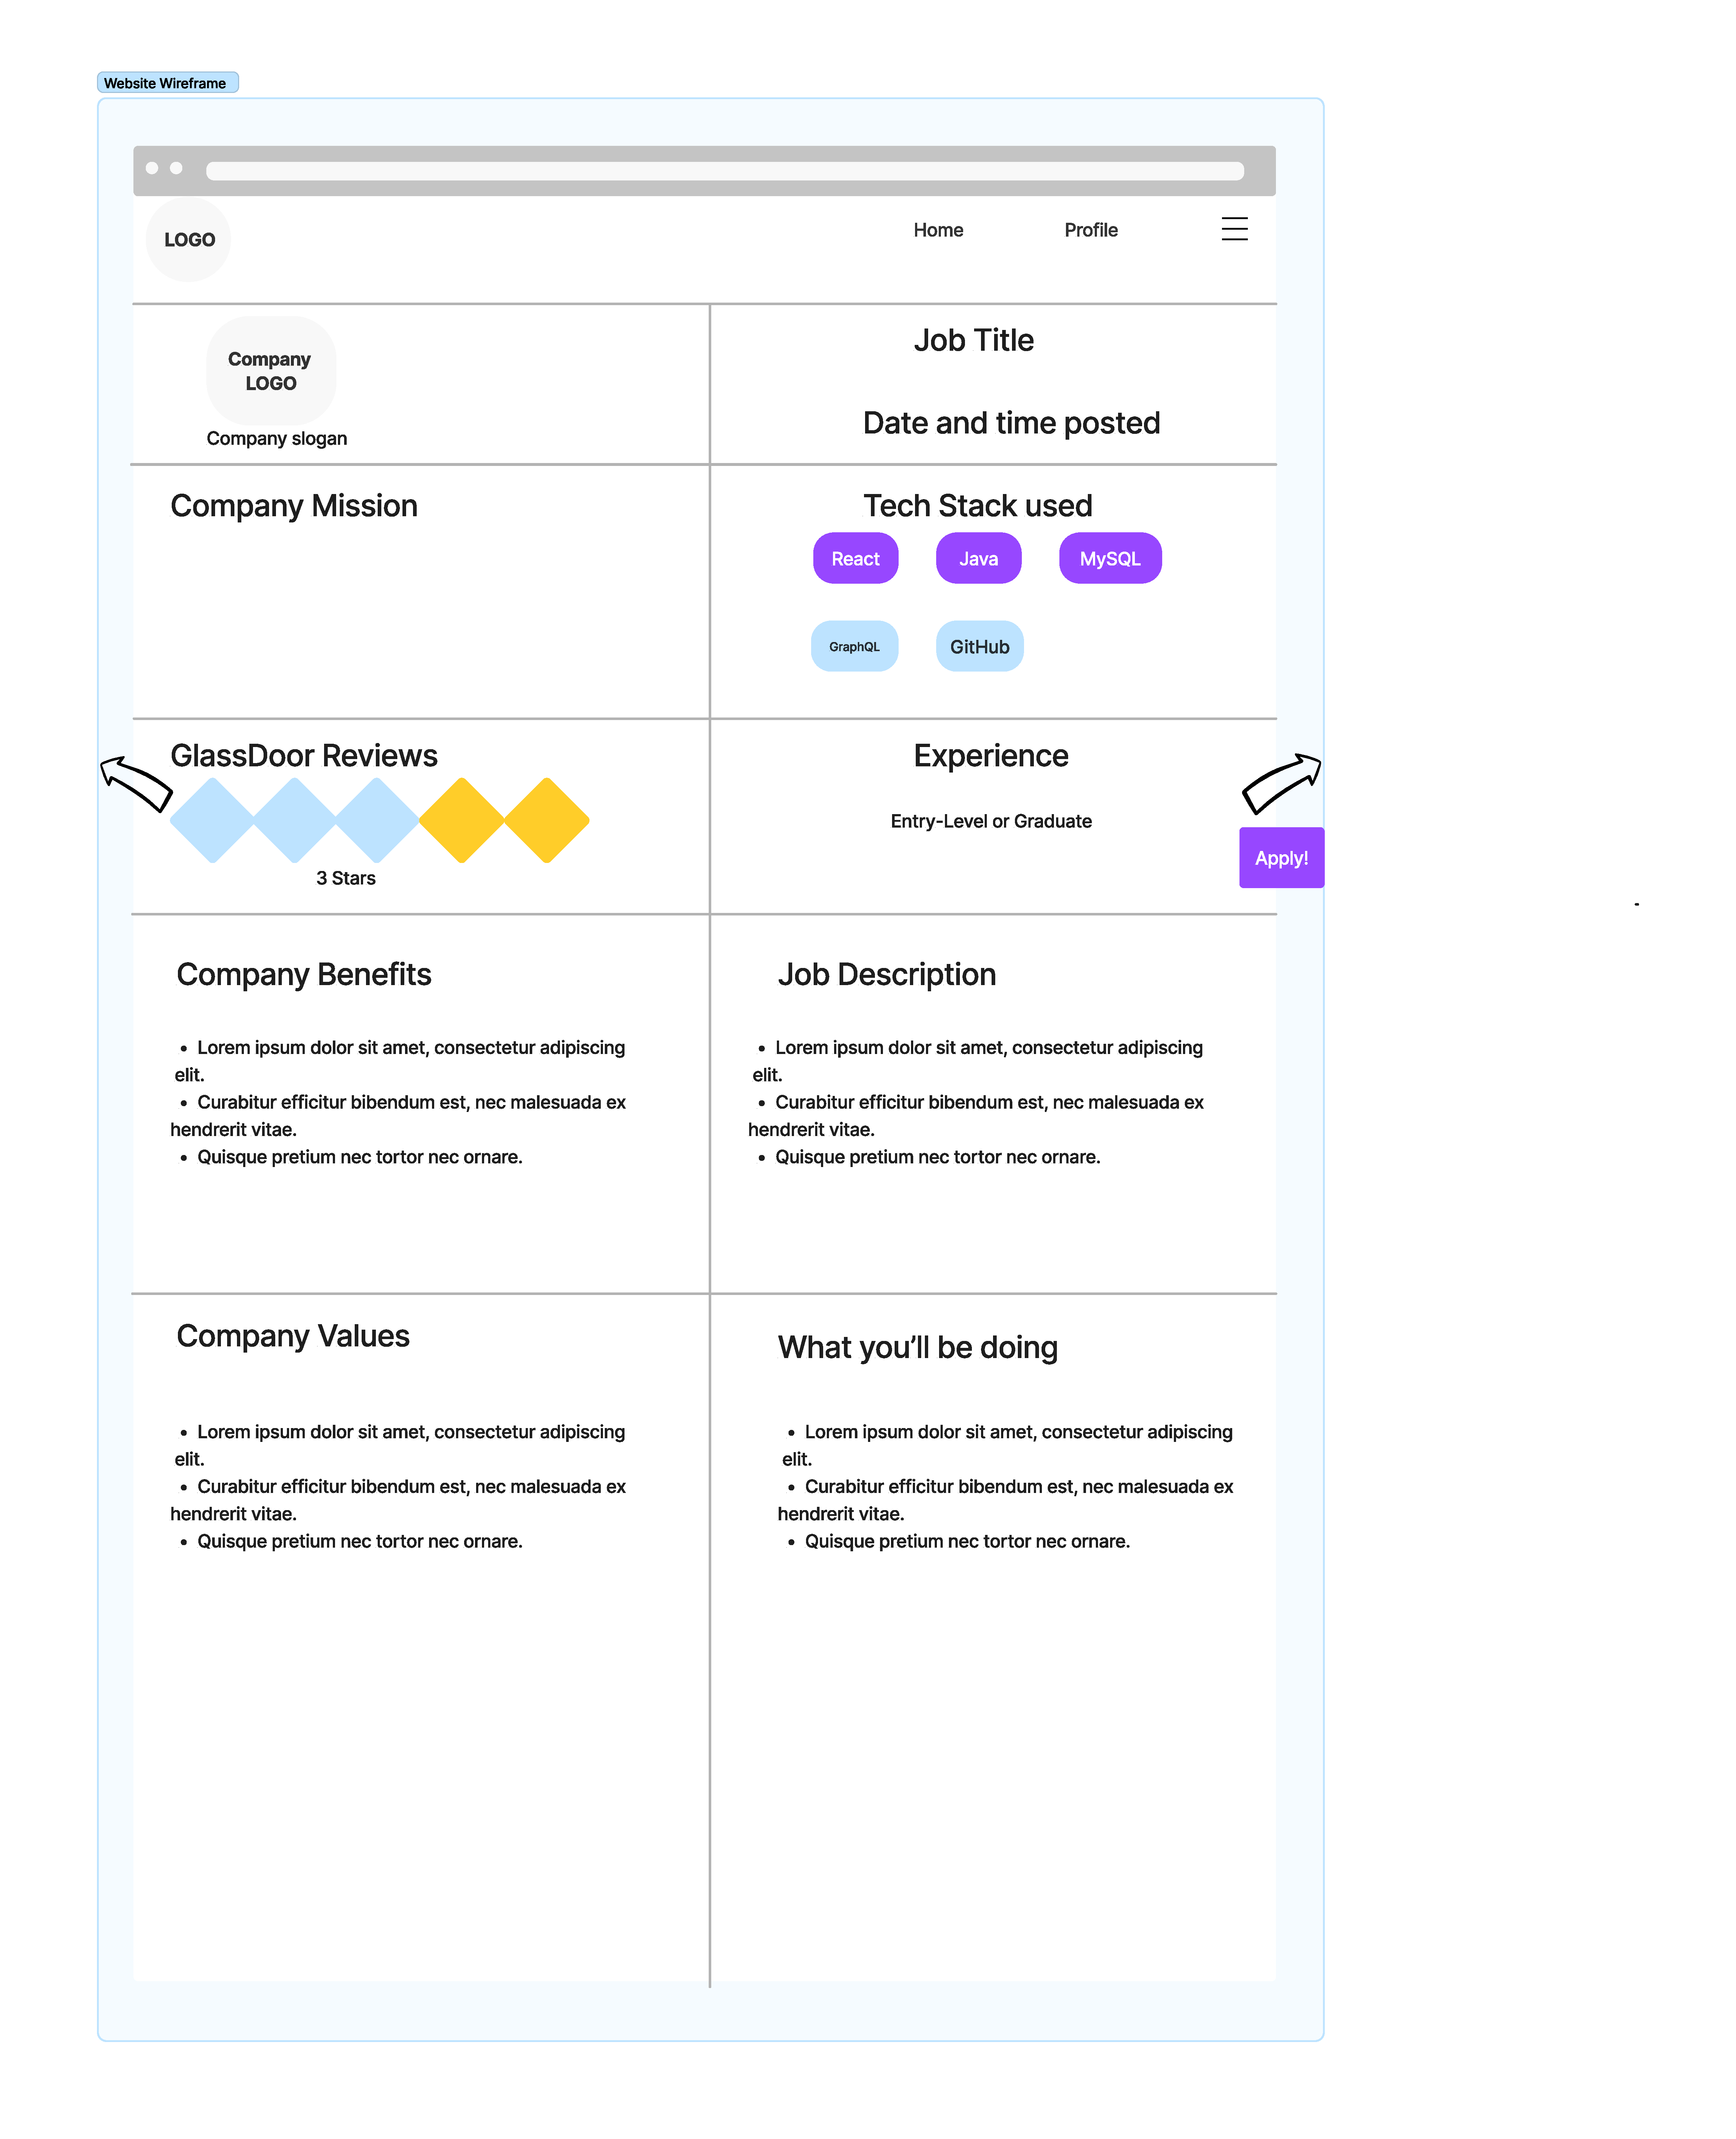
\includegraphics[width = 140mm]{Figures/posting.pdf}
    \decoRule
    \caption[Example of a job posting on the application]{Example of a job posting on the application}
    \label{fig: Job Posting}
\end{figure}

\begin{figure}
    \noindent
    \centering
    \includegraphics[width = 140mm]{Figures/loginPage.pdf}
    \decoRule
    \caption[Login Page]{Login Page}
    \label{fig: Login Page}
\end{figure}


\newpage
\section{Future Work}
While the first prototype of the designs is ready, they are not user-tested. These designs will be given to different users to provide feedback which will be noted and implemented in the future during the implementation of this application. 

As the implementation of this application is ongoing, multiple iterations will be done in the design, and as a result, the application's design will continue to change. Some things noted in the previous sections will also be worked on in the coming months, such as having similar colour choices throughout the application to make it more user-friendly. 

Testing is also one of the critical things that must be done in the Implementation stage. User Testing, Unit Testing, and Integration Testing are some tests which will be done in the implementation stage. 

Hosting the application will be done on the University Servers, and users will be able to provide feedback on the application by using it on their devices. This will prove beneficial as different devices using different browsers may have some errors which could be fixed during the implementation stage. 

In the MVP of this application, an employer should be able to add and create a new job posting, which the applicant should be able to see if their requirements meet the employers. All functional requirements should also be met for the MVP of this application.
%\include{Chapters/Chapter4} 
%\include{Chapters/Chapter5} 

%----------------------------------------------------------------------------------------
%	THESIS CONTENT - APPENDICES
%----------------------------------------------------------------------------------------

\appendix % Cue to tell LaTeX that the following "chapters" are Appendices

% Include the appendices of the thesis as separate files from the Appendices folder
% Uncomment the lines as you write the Appendices

% % Appendix A

\chapter{Frequently Asked Questions} % Main appendix title

\label{AppendixA} % For referencing this appendix elsewhere, use \ref{AppendixA}

\section{How do I change the colors of links?}

The color of links can be changed to your liking using:

{\small\verb!\hypersetup{urlcolor=red}!}, or

{\small\verb!\hypersetup{citecolor=green}!}, or

{\small\verb!\hypersetup{allcolor=blue}!}.

\noindent If you want to completely hide the links, you can use:

{\small\verb!\hypersetup{allcolors=.}!}, or even better: 

{\small\verb!\hypersetup{hidelinks}!}.

\noindent If you want to have obvious links in the PDF but not the printed text, use:

{\small\verb!\hypersetup{colorlinks=false}!}.

%\include{Appendices/AppendixB}
%\include{Appendices/AppendixC}

%----------------------------------------------------------------------------------------
%	BIBLIOGRAPHY
%----------------------------------------------------------------------------------------

\printbibliography[heading=bibintoc]

%----------------------------------------------------------------------------------------

\end{document}  
